\documentclass[review]{elsarticle}

\usepackage{hyperref}
\usepackage{lineno}
\modulolinenumbers[5]
\usepackage{amsmath}
\usepackage{graphicx}
\usepackage{booktabs}
\usepackage{url}
\usepackage{caption}
\usepackage{siunitx}
\usepackage{geometry}
\usepackage{multirow}
\usepackage{listings}
\usepackage{csvsimple}
\usepackage[T1]{fontenc}
\usepackage{hyphenat}
% \usepackage{underscore} % not needed; causes conflicts
\usepackage{enumitem}
\usepackage{prisma-flow-diagram}
\usepackage{placeins}

% PDF metadata and link styling
\hypersetup{
  colorlinks=true,
  linkcolor=blue,
  citecolor=blue,
  urlcolor=blue,
  pdftitle={WS3: An open-source Python framework for integrated simulation and optimization of forest landscape and wood supply systems},
  pdfauthor={Gregory Paradis},
  pdfsubject={Submitted to Ecological Informatics},
  pdfkeywords={computational ecology, decision support, forest planning, optimization, carbon accounting, geospatial workflows, open-source software}
}

\journal{Ecological Informatics}

\begin{document}

\begin{frontmatter}

\title{WS3: An open-source Python framework for integrated simulation and optimization of forest landscape and wood supply systems}

\author[ubc]{Gregory Paradis\corref{cor1}}
\cortext[cor1]{Corresponding author: gregory.paradis@ubc.ca}
\address[ubc]{Faculty of Forestry, University of British Columbia, Canada}

% Graphical abstract (optional)
\begin{graphicalabstract}
  \centering
  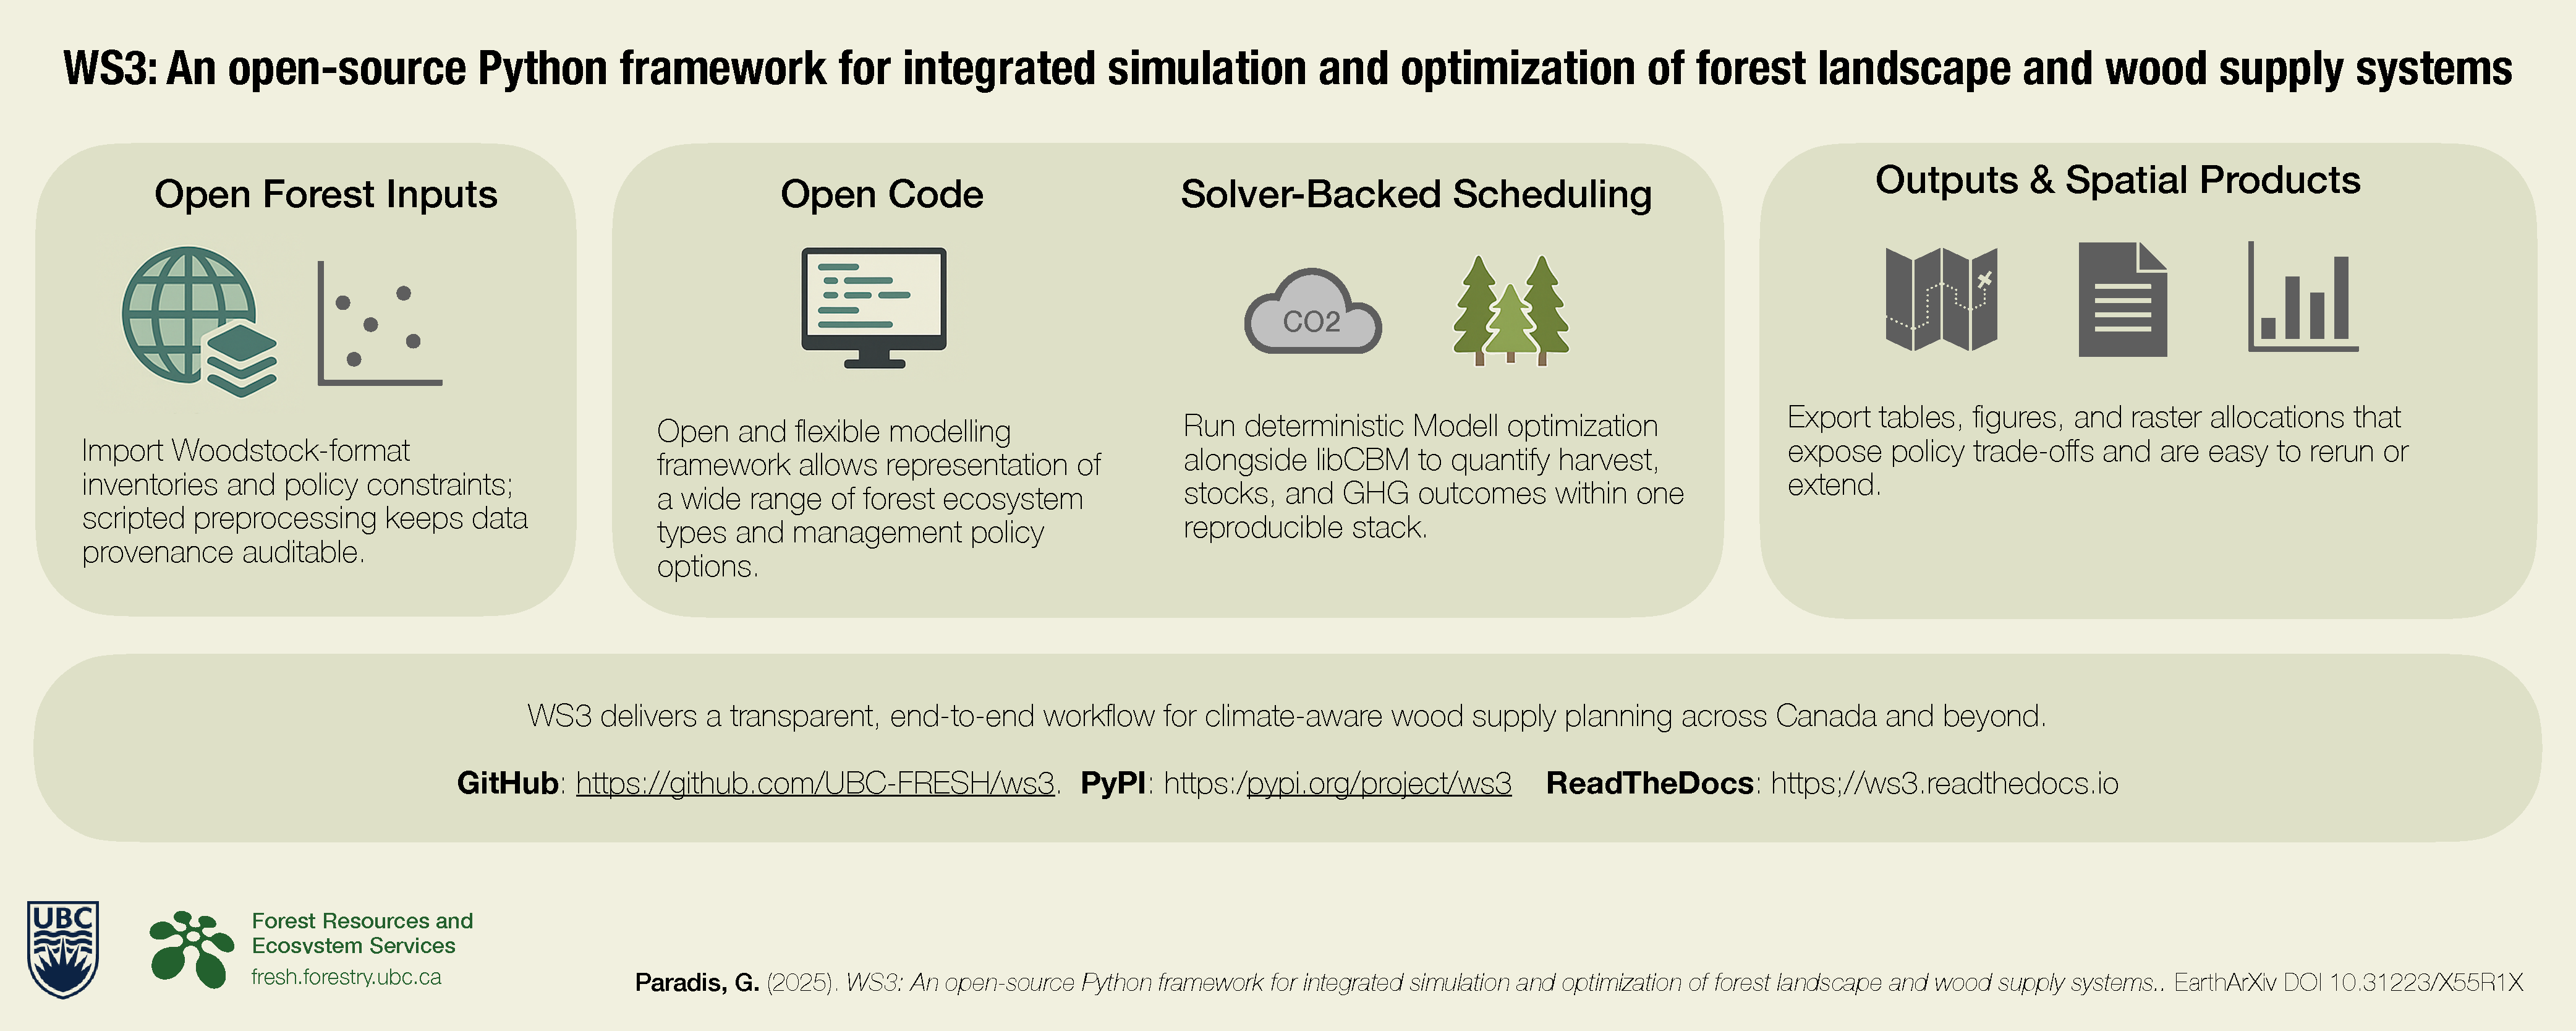
\includegraphics[width=\linewidth]{ws3-manuscript-graphical-abstract.pdf}
\end{graphicalabstract}

\section*{Highlights}
\begin{itemize}
  \item Open-source Python framework for forest estate decision support.
  \item Model~I scheduling with transparent inputs and outputs.
  \item libCBM linkage for carbon stock and flux accounting.
  \item Hybrid aspatial-to-raster workflows with reproducible geospatial I/O.
  \item Deterministic reproduction package and archived scaling benchmarks.
\end{itemize}

\begin{abstract}
WS3 is an open-source Python framework that integrates Model~I scheduling, carbon accounting, and raster allocation into a scriptable workflow for reproducible forest planning. It ingests Woodstock-format inventories, actions, and scenarios; defines an explicit data model; and automates aspatial--spatial conversion so harvest schedules can be mapped to disturbance footprints. A documented linkage to the Canadian Forest Service Carbon Budget Model (libCBM) provides carbon stock and flux estimates for libCBM-calibrated jurisdictions.

We document a modular architecture that decouples inventory ingestion, linear programming (LP) scheduling, carbon accounting, and raster allocation. Users can combine heuristic and LP approaches and extend indicators. We provide a reproducible parity check against Woodstock on a toy dataset and scaling experiments that characterize runtime and memory envelopes from desktop to cluster deployments. The complete toolchain---source code, configuration files, and deterministic reproduction scripts---is released under the MIT license with an archived Zenodo DOI. We demonstrate WS3 on five timber supply areas in northeastern British Columbia (20.40~Mha combined); post hoc libCBM runs provide carbon trajectories and raster allocation produces disturbance footprints for downstream spatial simulators. The framework is intended as reusable informatics infrastructure for decision support under competing sustainability mandates.
\end{abstract}

\begin{keyword}
computational ecology \sep decision support \sep forest planning \sep optimization \sep carbon accounting \sep geospatial workflows \sep open-source software
\end{keyword}

\section*{Software availability}
\begin{itemize}
  \item Software name: WS3 (Wood Supply Simulation System)
  \item Developer and contact: Gregory Paradis (Faculty of Forestry, University of British Columbia); \href{mailto:gregory.paradis@ubc.ca}{gregory.paradis@ubc.ca}
  \item First public release and current version: 2015 (v0.1); current release v1.0.5
  \item Programming language and dependencies: Python (>=3.9); optional extras include \texttt{libcbm\_py} (Carbon Budget Model Python bindings), PuLP (Python LP modeling) with the HiGHS solver, and Gurobi
  \item Source repository and issue tracker: \url{https://github.com/UBC-FRESH/ws3}
  \item Distribution channel: PyPI package \texttt{ws3} (\texttt{pip install ws3} or \texttt{ws3[cbm]}) with wheels for Linux, macOS, and Windows
  \item Documentation: \url{https://ws3.readthedocs.io}
  \item Archived release: Zenodo DOI \href{https://doi.org/10.5281/zenodo.17331213}{10.5281/zenodo.17331213}
  \item License: MIT
  \item Hardware and OS requirements: Linux, macOS, or Windows; tested on Ubuntu 24.04 and macOS 14; CPU-only with recommended 16+ GB RAM for large LP instances
  \item Tested Python versions: 3.9--3.12 (continuous integration matrix)
  \item Data form and access: supplementary CSV, GeoTIFF, and notebook artifacts packaged in the GitHub repository and Zenodo release; total archive size under 50 MB excluding optional outputs
\end{itemize}

\end{frontmatter}

\clearpage

\linenumbers

\section{Introduction}

Forested landscapes sit at the center of intertwined climate mitigation, biodiversity, and bioeconomy mandates. Planners are being asked to reconcile wood supply security with measurable reductions in greenhouse-gas emissions across multi-decadal horizons \citep{canadell2022wgiii, griscom2017natural, fao2020fra}. Meeting these expectations demands decision-support systems that span harvest scheduling, regeneration and silviculture options, spatial footprint analysis, and explicit carbon accounting, while remaining transparent enough for regulators, Indigenous governments, and industrial partners to audit \citep{law2018land, smyth2020climate}. This analytical load has outgrown the ad hoc spreadsheets and siloed software stacks that remain common in practice. It underscores the need for integrated modeling platforms that support reproducible workflows and open-science norms, including the PERFICT reproducibility principles for predictive ecology---a checklist for transparent, reusable computational workflows \citep{hampton2015tao, lowndes2017path, mcintire2022perfict}.

Strategic forest planning has long relied on operations research formulations such as Model~I path scheduling and its variants, which underpin allowable-cut analyses and forest estate studies worldwide \citep{johnson1977techniques, gunn2007models, gunn2009some, paradis2013risk}. Model~I is a strata-based linear program in which decision variables assign fractions of aggregated development-type strata to prescriptions over time; this enables large-scale policy analysis but necessarily abstracts away stand identities. In practice, these ideas are delivered through proprietary toolchains---Woodstock, Patchworks, JLP (MELA), and Heureka, among others---that package data models, solvers, and reporting inside closed desktop environments \citep{remsoft-woodstock, patchworks, jlp_mela, heureka}. These systems are mature and widely trusted, yet closed licensing and opaque configuration formats can limit transparency, collaborative extension, and reproducible research workflows increasingly required by regulators and journals \citep{hampton2015tao}.

Open-source platforms have begun to address parts of this gap. Spatial simulation systems such as SpaDES and LANDIS-II, scenario-management frameworks like SyncroSim, and planning prototypes such as PRISM provide modular, shareable tooling \citep{spades, landisii, syncrosim, nguyen2022prism}. These systems excel at spatial dynamics and scenario orchestration but typically require users to supply planning modules, solver integrations, and carbon accounting pipelines to assemble a full decision-support stack \citep{daigneault2022forest, law2018land}. Parallel efforts such as the French CAPSIS platform highlight the promise and complexity of interoperable forest growth modeling ecosystems \citep{fortin2022altframework, fortin2022metamodel, power2015artemis}. This gap between open simulation scaffolds and end-to-end forest estate planning motivates the framework described here.

WS3 is an open Python framework that implements legacy Model~I scheduling while emphasizing reproducible, scriptable workflows with carbon accounting. It imports Woodstock-format text files (or equivalent information in \emph{ad hoc} formats via custom Python parsers) to protect historical investments, supports multiple LP solvers, couples to the Canadian Forest Service libCBM implementation, and supports hybrid spatial--aspatial workflows compatible with geospatial rasters and SpaDES-based simulations \citep{remsoft-woodstock, pulp, highs, gurobi, kurz2009cbm, libcbm_py, spades}. We do not claim a new optimization formulation; rather, we provide a transparent and auditable implementation that can be inspected, extended, and reproduced across institutions \citep{hampton2015tao, lowndes2017path}.

This article contributes to ecological informatics in three ways. First, it documents a modular decision-support architecture that combines harvest scheduling, carbon accounting, and spatial reporting in a single, scriptable workflow. Second, it provides evidence of functional parity with Woodstock on a toy dataset and reports computational scaling experiments that characterize runtime and memory envelopes for large landscapes. Third, it makes the complete toolchain—source code, configuration files, and reproduction scripts—available under an open license with an archived Zenodo DOI, enabling immediate reuse and extension by researchers and practitioners. These contributions are workflow- and reproducibility-oriented; we do not propose a new optimization formulation.

The remainder of this article details the WS3 architecture and data model (Section~2), demonstrates reproducible use-case workflows linking LP-based scheduling to libCBM carbon accounting and spatial disturbance allocation (Section~3), discusses scope and limitations (Section~4), compares WS3 with alternative tools (Section~5), and summarizes availability, authorship, and future work to facilitate uptake.

\section{Software description}
\subsection{Architecture}
WS3 is organized into five roles: (i) core data abstractions; (ii) forest model construction and simulation; (iii) optimization; (iv) spatial allocation; and (v) common utilities. The main modules are:
\begin{itemize}
  \item \texttt{forest}: defines the ForestModel and core abstractions for development types (dtypes), actions, transitions, yields, and scenario compilation. A scenario is specified by a planning horizon, period length, an initial inventory (areas by dtype and age), and transition rules governing state changes under actions and growth.
  \item \texttt{opt}: provides a linear-programming (LP) interface to formulate harvest-scheduling problems (objective, variables, constraints) and to solve them via PuLP with HiGHS by default; optional Gurobi.
  \item \texttt{spatial}: maps aspatial schedules to rasters (e.g., GeoTIFF) for visualization and spatial policy evaluation in a hybrid spatial/aspatial workflow.
  \item \texttt{core}, \texttt{common}, \texttt{financial}, \texttt{forest\_helper}: shared utilities for interpolation and curves, example helpers, and optional financial indicators.
\end{itemize}

\emph{Data model and workflow.} The ForestModel class uses discrete time (planning periods) and discrete age classes per dtype. Dtypes are keyed by tuples of theme values (e.g., analysis unit, leading species, site class). For optimization, WS3 aggregates stands into strata defined by dtype and optional zone masks (e.g., management units or policy zones). Spatial units (stands, polygons, or raster cells) appear only in the allocation step. Yields are represented by curves or interpolators. Actions (e.g., harvest, planting, fuel treatment, fire) encode operability and transitions (age reset, development type change, growth updates). WS3 builds a state-transition tree per development type across periods. Scheduling can be heuristic (area-control selectors that meet target areas by mask in priority order, e.g., oldest-first) or solver-based via a generic Model~I linear program. Indicators are compiled as:
\begin{itemize}
  \item Action-dependent flows via \texttt{compile\_product(period, expr, acode=...)} (e.g., harvested volume using a utilization-adjusted expression on total volume yield).
  \item Inventory stocks via \texttt{inventory(period, yname=...)} (e.g., growing stock).
\end{itemize}

\emph{Interoperability}. WS3 imports Woodstock-format text sections (LANDSCAPE, AREAS, YIELDS, ACTIONS, TRANSITIONS) so existing pipelines can be reused without re-encoding model logic. For carbon, ForestModel provides \texttt{to\_cbm\_sit} to export Standard Input Table (SIT) configuration and tables consumable by libCBM; users supply disturbance-type mappings and per-dtype last-pass-disturbance metadata. libCBM ships with parameterizations for multiple countries and ecozones \citep{kurz2009cbm}, so the same export pathway supports analyses beyond Canada when users supply the appropriate classifiers and disturbance libraries. Geospatial I/O uses standard formats (shapefile, GeoTIFF). All tabular inputs are plain text (CSV/TSV), and workflows are scripted or notebook-based for reproducibility.

Figure~\ref{fig:workflow_overview} summarizes the WS3 workflow from open inputs through scheduling, carbon analysis, and spatial reporting. The end-to-end case study pipeline is implemented in the reproduction package and described below.

\begin{figure}[h]
  \centering
  \resizebox{\textwidth}{!}{
  \prismaflowstart
  % Inputs row
  \prismaflownode{in1}{below=of tc}{\textbf{Inventory}\\Yields, areas, themes}{}
  \prismaflownode{in2}{right=of in1}{\textbf{Actions \& transitions}}{}
  \prismaflownode{in3}{right=of in2}{\textbf{Scenario config}\\CSV / YAML}{}
  \prismalabel{1.3*\mh}{in1.west}{Inputs}

  % WS3 core row
  \prismaflownode{core1}{below=of in2}{\textbf{ForestModel}\\Data API}{in2}
  \prismaflownode{core2}{below=of core1}{\textbf{Optimization}\\PuLP / HiGHS / Gurobi}{core1}
  \prismaflownode{core3}{right=of core2}{\textbf{Simulation \& reporting}}{core2}
  \prismalabel{1.3*\mh}{in1.west |- {$(core1)!0.5!(core2)$}}{WS3 core}

  % Integration row
  \prismaflownode{int1}{below=of core2}{\textbf{libCBM}\\Carbon pools \& flux}{core2}
  \prismaflownode{int2}{right=of int1}{\textbf{Spatial allocation}\\Rasterio / GeoTIFF}{core3}
  \prismalabel{1.3*\mh}{in1.west |- int1}{Integrate}

  % Outputs row
  \prismaflownode{out1}{below=of int1}{\textbf{Outputs}\\Dashboards, reports, reproducible assets}{int1}
  \prismalabel{1.3*\mh}{in1.west |- out1}{Outputs}

  % Arrows from inputs
  \prismaflowarrow{in1}{core1}
  \prismaflowarrow{in2}{core1}
  \prismaflowarrow{in3}{core1}

  % Arrows to integration
  %\prismaflowarrow{core1}{int1}

  % Arrows to outputs
  \prismaflowarrow{int2}{out1}

  \prismaflowend
  }
  \caption{WS3 workflow: categorized inputs feed core scheduling and reporting modules, which integrate with libCBM and spatial allocation utilities before producing reproducible outputs.}
  \label{fig:workflow_overview}
\end{figure}

The case study workflow implemented in the reproduction package loads Woodstock-format inputs, constructs the \texttt{ForestModel} instance, computes a schedule (heuristic or LP-based), exports a libCBM Standard Input Table formatted dataset, runs libCBM, allocates the aspatial schedule to raster space, and generates the figures and tables. This scripted pipeline underpins the sequential case study documented in Section~\ref{sec:usecase}. Note that WS3 is flexible and has been used in many workflows; the intent of the case study workflow shown here is illustrative rather than prescriptive or restrictive.

\begin{figure}[t]
  \centering
  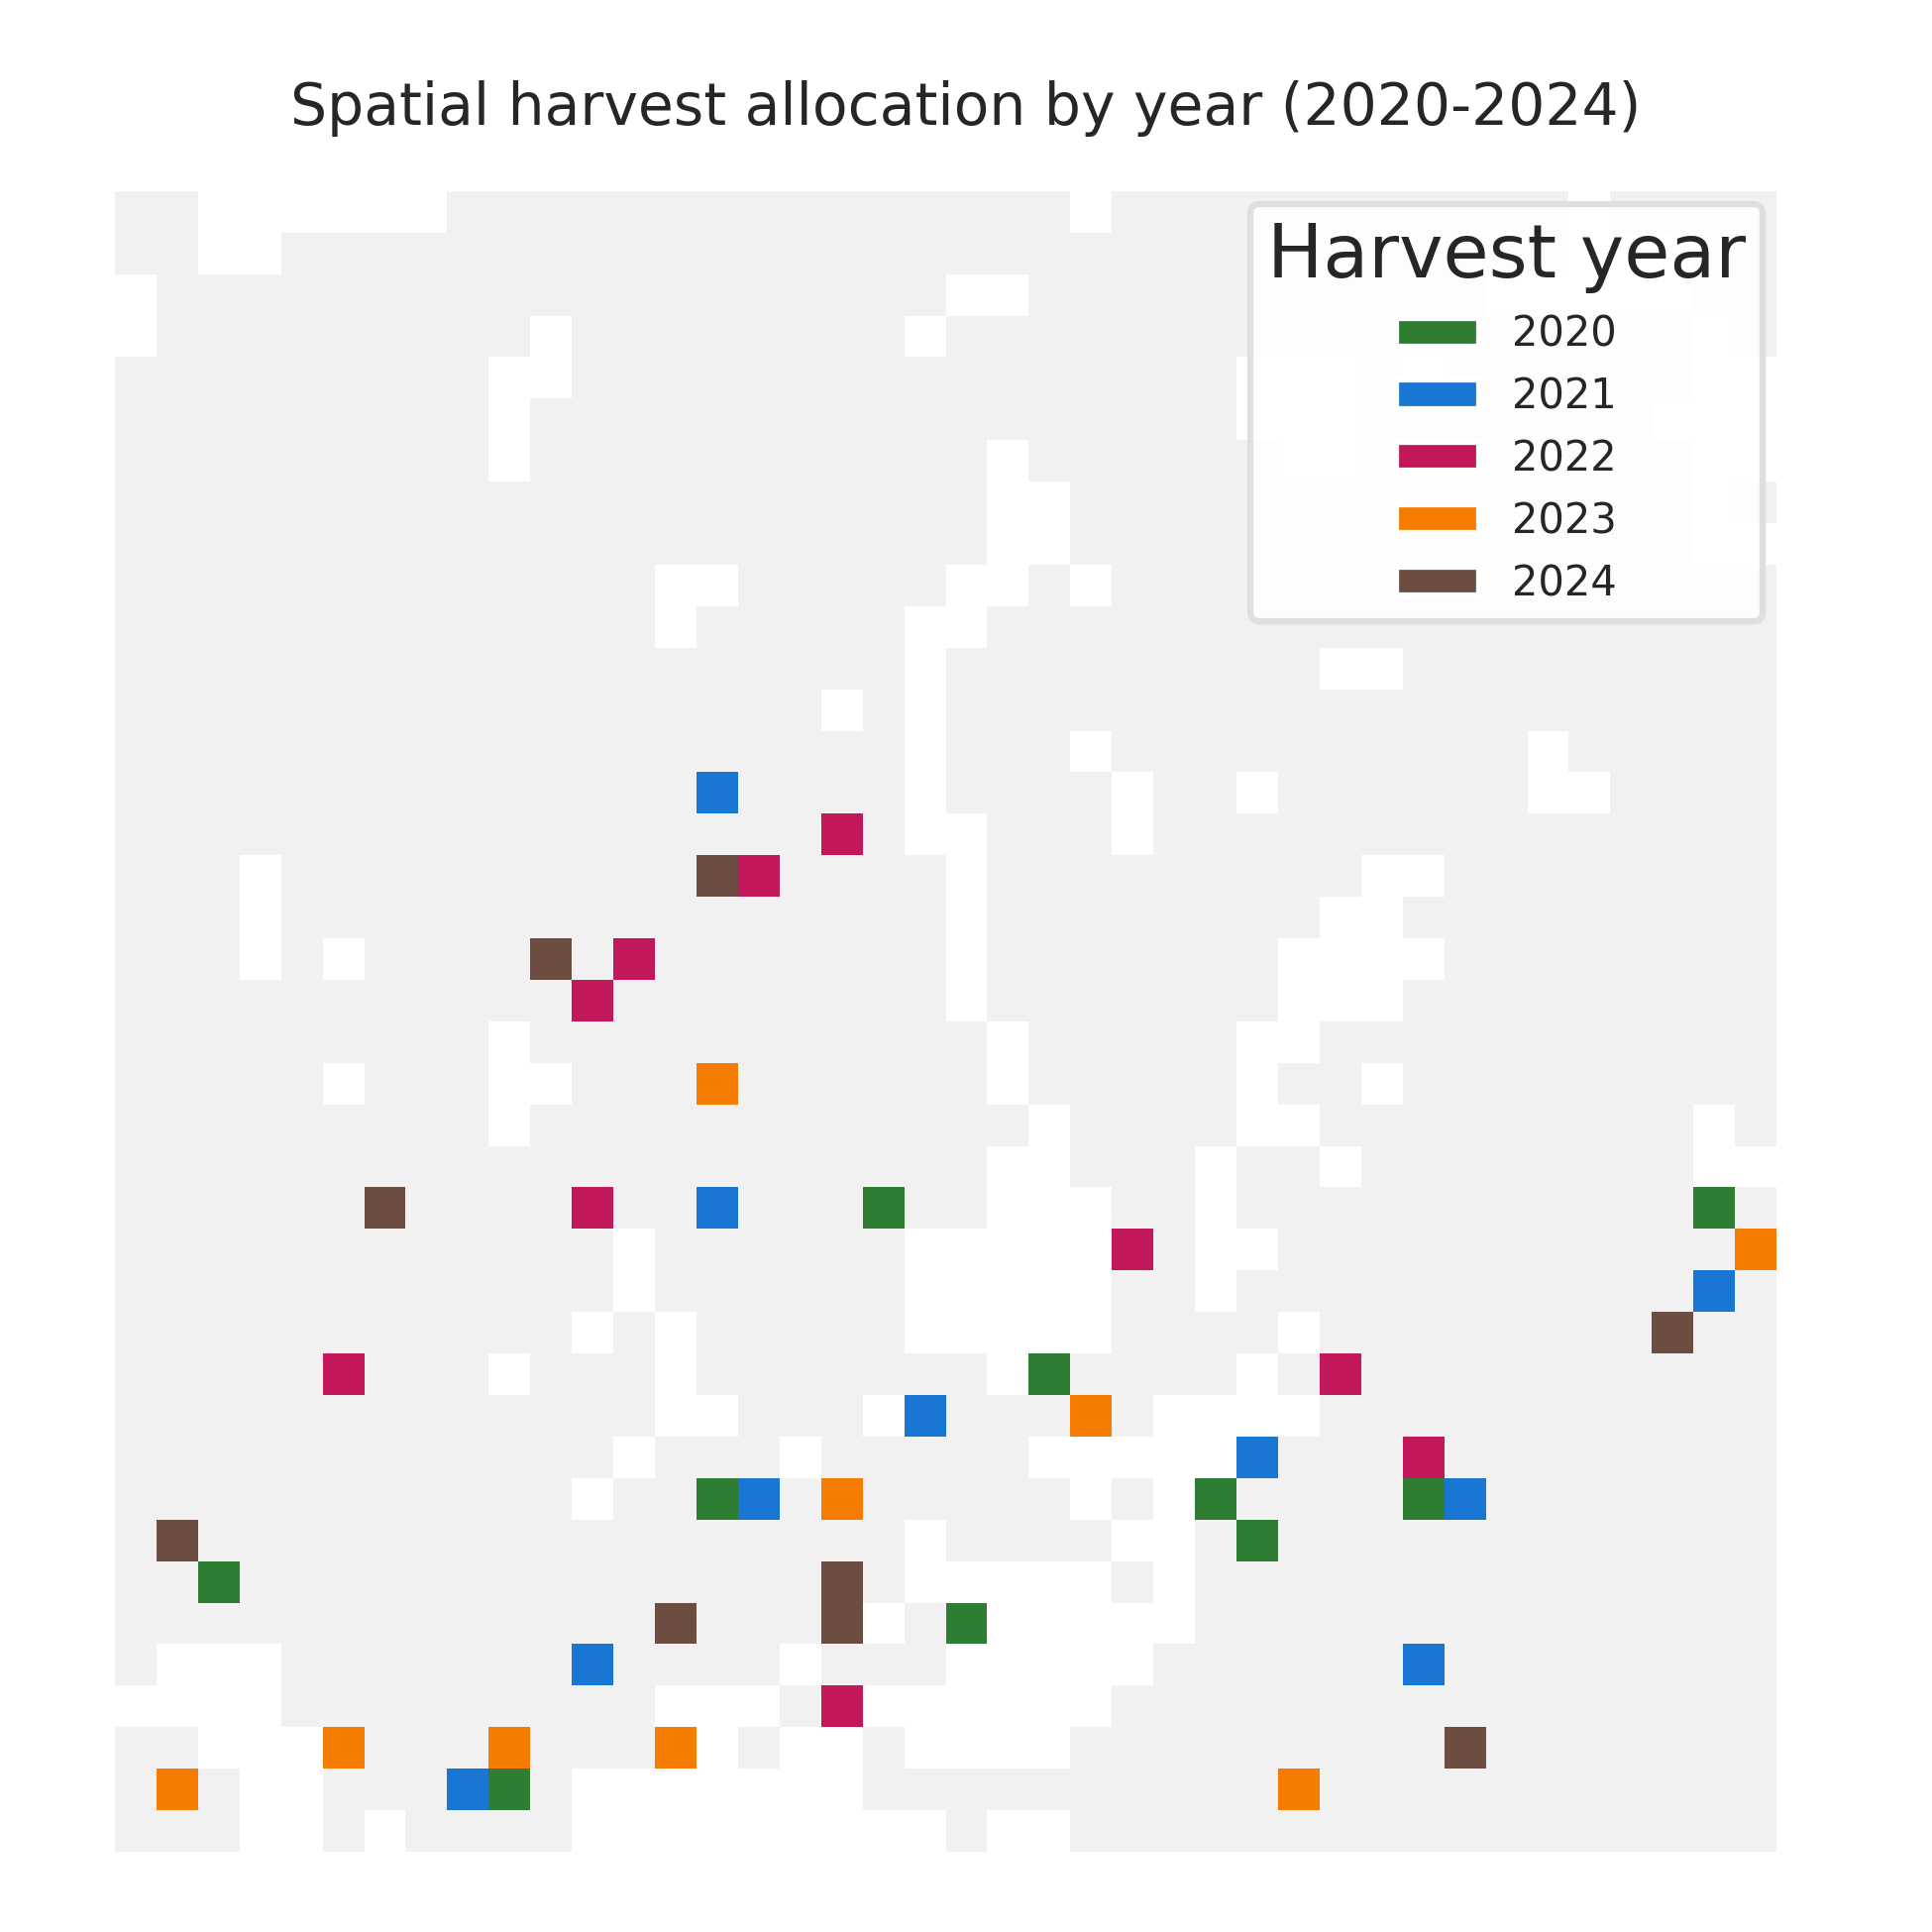
\includegraphics[width=0.7\linewidth]{figs/f3_spatial_allocation.png}
  \caption{Heuristic schedule allocated to space for the 2020--2024 planning window. Colours denote the first year a cell is harvested, overlaid on the full inventory extent (light grey).}
  \label{fig:spatial_allocation}
\end{figure}

We summarize four practical contributions:
\begin{enumerate}[label=(\roman*)]
  \item A solver-flexible, path-based Model~I generator embedded within a documented forest estate API, with parallel coefficient compilation for large instances.
  \item A documented libCBM interface that exports Standard Input Tables and ingests carbon pools and fluxes for integrated accounting.
  \item A hybrid aspatial-to-raster allocation workflow that emits reproducible geospatial artifacts from deterministic schedules.
  \item A FAIR-aligned reproduction package, including scaling benchmarks on real inventories and archived releases with pinned environments.
\end{enumerate}

\FloatBarrier

\subsection{Optimization formulation (Model~I)}
WS3 adopts a classic Model~I linear programming formulation \citep{johnson1977techniques, gunn2007models} in which each decision variable selects the proportion of a stratum (a dtype aggregate, optionally intersected with a zone mask) allocated to a feasible root-to-leaf prescription (path) across the planning horizon. Stand identities are aggregated into strata for optimization, and spatial allocation is handled separately. Let:
\begin{align*}
  I &: \text{ set of strata (development types; aggregated zones)} \\
  J_i &: \text{ set of feasible prescriptions (paths) for stratum } i\in I \\
  O &: \text{ set of outputs (e.g., harvest area, harvest volume, growing stock, habitat)} \\
  O'&\subseteq O: \text{ targeted outputs subject to even-flow constraints} \\
  T &: \text{ set of planning periods} \\
  T'_p&\subseteq T: \text{ periods on which even-flow for output } p\in O' \text{ is enforced}
\end{align*}
Decision variables are proportions:
\[
x_{ij}\in[0,1] \quad \text{for all } i\in I,\, j\in J_i,
\]
representing the fraction of stratum $i$ assigned to prescription $j$. If $A_i$ denotes the total area in stratum $i$, then $A_i x_{ij}$ is the area scheduled on path $j$. Let $\mu_{ijot}$ denote the quantity of output $o\in O$ in period $t\in T$ produced by allocating $x_{ij}$ to path $j\in J_i$ for stratum $i\in I$. Define the reference-period output level $y_p:=\sum_{i\in I}\sum_{j\in J_i}\mu_{ij p t_p^R}x_{ij}$ for each targeted output $p\in O'$ at $t_p^R\in T$, and $\varepsilon_p$ as the allowable even-flow tolerance. With general lower/upper bounds $v^-_{ot},v^+_{ot}$ on outputs, the Model~I LP is:
\begin{align}
\text{maximize}\quad
& \sum_{i\in I}\sum_{j\in J_i} c_{ij}\,x_{ij} \label{eq:ws3_obj}\\
\text{subject to}\quad
& (1-\varepsilon_p)\,y_p \le \sum_{i\in I}\sum_{j\in J_i}\mu_{ijpt}\,x_{ij} \le (1+\varepsilon_p)\,y_p, && \forall p\in O',\, \forall t\in T'_p \label{eq:ws3_evenflow}\\
& v^-_{ot} \le \sum_{i\in I}\sum_{j\in J_i}\mu_{ijot}\,x_{ij} \le v^+_{ot}, && \forall o\in O,\, \forall t\in T \label{eq:ws3_bounds}\\
& \sum_{j\in J_i} x_{ij} = 1, && \forall i\in I \label{eq:ws3_coverage}\\
& 0 \le x_{ij} \le 1, && \forall i\in I,\, \forall j\in J_i. \label{eq:ws3_box}
\end{align}
The objective coefficients $c_{ij}$ encode the user-defined value of a path (e.g., total or discounted volume, revenues, multi-criteria scores). Constraints (\ref{eq:ws3_evenflow}) enforce even-flow on targeted outputs, (\ref{eq:ws3_bounds}) set general lower/upper bounds per period, (\ref{eq:ws3_coverage}) ensures convex mixing of paths to fully cover each stratum, and (\ref{eq:ws3_box}) bounds variables as proportions. In WS3, $\mu$-coefficients arise from replaying each path through the simulator, calling \texttt{compile\_product} (action-dependent outputs such as harvest area and volume) or \texttt{inventory} (stocks such as growing stock). The LP matrix is sparse because each path contributes to a limited set of outputs and periods.

\emph{Code-to-math mapping.} WS3 compiles objective and constraint rows from paths using coefficient functions. Helper routines (e.g., \texttt{cmp\_c\_z}, \texttt{cmp\_c\_caa}, \texttt{cmp\_c\_ci}) traverse path nodes (period, action code, dtype key, age), evaluate $\mu$-like contributions via \texttt{compile\_product}/\texttt{inventory}, and assemble the LP with \texttt{fm.add\_problem(...)}. Users select a solver (HiGHS by default; Gurobi optional) and solve via the standard PuLP interface. Upon optimality, WS3 applies the schedule and re-simulates to produce indicators.

\emph{Design implications.} This path-based Model~I approach embeds intertemporal feasibility in each column, separates simulation from optimization, and enables straightforward addition of new outputs/constraints by supplying new coefficient functions. It also aligns with established forest-planning literature while remaining solver-flexible and highly sparse for scalability.

\subsection{Implementation}
\emph{Technology stack.} WS3 is implemented in Python and distributed via PyPI. Optimization problems are formulated by WS3 and solved with the open-source HiGHS \citep{highs} solver by default through the PuLP \citep{pulp} Python LP interface, with optional Gurobi \citep{gurobi} bindings. Geospatial I/O uses rasterio, fiona, and GeoPandas. Documentation (Sphinx) and continuous integration (CI) pipelines provide API checks, runnable examples, and unit tests.

\emph{libCBM integration.} The ForestModel class provides a \texttt{to\_cbm\_sit} method that compiles a CBM Standard Input Table (SIT) configuration and table data structure (i.e., classifiers, inventory, yields, disturbance events, transitions) consumable by libCBM. Users provide a disturbance type mapping and last-pass disturbance metadata to ensure correct dead organic matter (DOM) spin-up. The sequential demonstration runs libCBM for 200 years using the official Python API and documentation \citep{libcbm_py_docs, libcbm_py_repo}.

\emph{Reproducibility and packaging.} The repository includes examples and a reproduction package (\path{papers/ems/repro}) with pinned requirements and scripts to generate all figures and tables. Versioned releases are archived on Zenodo \citep{ws3_zenodo2025}. WS3 supports interactive (Jupyter notebooks) and batch (Python scripts) workflows and can be embedded in other systems as a standard Python dependency.

\subsection{Quality assurance and benchmarking}
\emph{Automated testing.} WS3 ships with a pytest suite that exercises the common, core, financial, forest, and optimization modules (29 tests). The suite runs in about 4~s on a Linux workstation (Python~3.12) and is executed for every push and pull request via a GitHub Actions workflow (Ubuntu, Python~3.10) that also regenerates a coverage badge \citep{ci_workflow}. Style tooling (Black, Ruff) is bundled in \texttt{requirements-dev.txt} and wired into the development Makefile, ensuring consistent formatting before release. Beyond unit tests, WS3 has been exercised in multiple operational planning projects over the past decade, providing repeated end-to-end validation of core workflows.

\emph{Input stewardship and validity.} WS3, like its Woodstock heritage, makes no assumptions about inventories, yields, operability, objectives, or constraints. The space of ``valid input'' is project- and policy-specific and inherently high-dimensional; exhaustive auto-validation is out of scope. WS3 provides targeted checks in high-leverage paths (e.g., fallback to template transitions when age-specific rules are missing; basic range/shape sanity checks) and documentation of required structures for inventories, yields, actions, and transitions. Documentation is versioned with releases and focuses on core data structures and examples rather than serving as an exhaustive prescriptive manual. Responsibility for input quality and modeling assumptions rests with qualified analysts; WS3 is a professional framework rather than a prescriptive application.

\emph{Determinism and reproducibility.} Given identical inputs, WS3 produces identical outputs. Minor nondeterminism is limited to optional solver seeds and randomized block ordering in the spatial allocation utility; both are controllable and fixed in the reproduction scripts. Consequently, statistical variance on deterministic time series is not meaningful; we report solved status, model scale, and runtime/throughput metrics instead. The reproduction package pins versions and seeds to yield byte-identical artifacts across runs, reflecting best practices for computational reproducibility \citep{peng2011reproducible}.

\emph{Verification against Woodstock.} WS3 was originally verified against Woodstock (2015) by replaying identical datasets and comparing action-specific flows and stocks across periods, yielding functionally equivalent outputs for the implemented subset of features. Known departures from Woodstock semantics are flagged in code and documentation. Ongoing development follows a trust-but-verify pattern: changes to core loops are regression-tested against known-good benchmarks before release. The Woodstock parity check included in this manuscript is therefore a transparent, reproducible illustration rather than an exhaustive proof of equivalence.

\emph{Case study repro checks.} The reproduction package encapsulates the sequential WS3$\to$libCBM pipeline in \texttt{make\_repro.sh}. In the project’s reference LXD (Linux Containers) environment (Ubuntu~24.04 on dual Xeon~6254 CPUs, 72 logical cores, 768~GB PC-23400 RAM) the script completes in 6.1~s, recreating Figures~\ref{fig:flows} and~\ref{fig:cbm}, Figure~\ref{fig:spatial_allocation}, and the summary tables. The workflow is deterministic: running \texttt{generate\_case\_study.py} a second time produces byte-identical CSV and PNG assets, providing an integration test for the scheduling, SIT export, and libCBM coupling.

\emph{Performance spot checks.} The heuristic scheduler used in the case study produces a 100-year plan in under a second, and the subsequent 200-year libCBM simulation dominates total runtime (\textasciitilde5~s). Larger linear programs formulated through \texttt{ws3.opt} benefit from HiGHS (default) or optional Gurobi: internal regression notebooks (e.g., Examples~030/040) solve tens of thousands of stand-path instances within minutes using HiGHS, and the optional Gurobi backend can reduce solve time further when available. Raster allocations scale linearly with the number of cells processed per period and can be parallelized by splitting periods or tiles.

\emph{Optional scalability experiment.} To characterize scaling on real inventories, the reproduction package optionally integrates a DataLad-hosted benchmark dataset comprising five non-overlapping timber supply areas (TSAs) in northeastern British Columbia (the same study region as \citealt{boisvenue2022managing}). Enabling the optional step (\texttt{RUN\_SCALING=1}) fetches the dataset and executes \texttt{papers/ems/repro/run\_scaling\_benchmarks.py}, which sorts TSAs by complexity and evaluates them individually and cumulatively (\texttt{tsa08}, \texttt{tsa08+tsa40}, \ldots, \texttt{tsa08+tsa40+tsa41+tsa24+tsa16}). The scripted benchmark always runs the heuristic scheduler single-threaded---reflecting the implementation's serial design---and records serial spatial-allocation runtimes using \texttt{ForestRaster}. On the reference container the heuristic schedules complete in 1.3--31.4~s while spatial allocation requires 46--656~s as problem size grows from 4.7~k to 37.7~k dtype--age pairs.

Setting \texttt{RUN\_LP=1} extends the run to model-building benchmarks for the deterministic Model~I LP. WS3 constructs the LP with 1 and 16 workers (parallel coefficient compilation) and solves it with matching HiGHS thread counts, logging build/solve time, solver status, and stage-wise memory footprints. LP builds scale from 5.1~s (4.7~k dtype--age pairs) to 92.8~s (37.7~k dtype--age pairs) with single-worker compilation, while the 16-worker mode trims build time to 59~s at the cost of higher peak resident set size (RSS; 2.5~GB versus 1.8~GB). Because large path-based LPs routinely exceed tens of gigabytes of RAM on even larger inventories, the LP measurements are opt-in and intended for suitably provisioned systems. All metrics are written to \texttt{perf\_scaling.csv} with deterministic seeds so that regenerated figures and tables remain byte-identical; Figures~\ref{fig:scaling_sched}--\ref{fig:scaling_mem} and~Table~\ref{tab:scaling_summary} summarize the resulting runtime and memory profiles.

\begin{figure}[h]
  \centering
  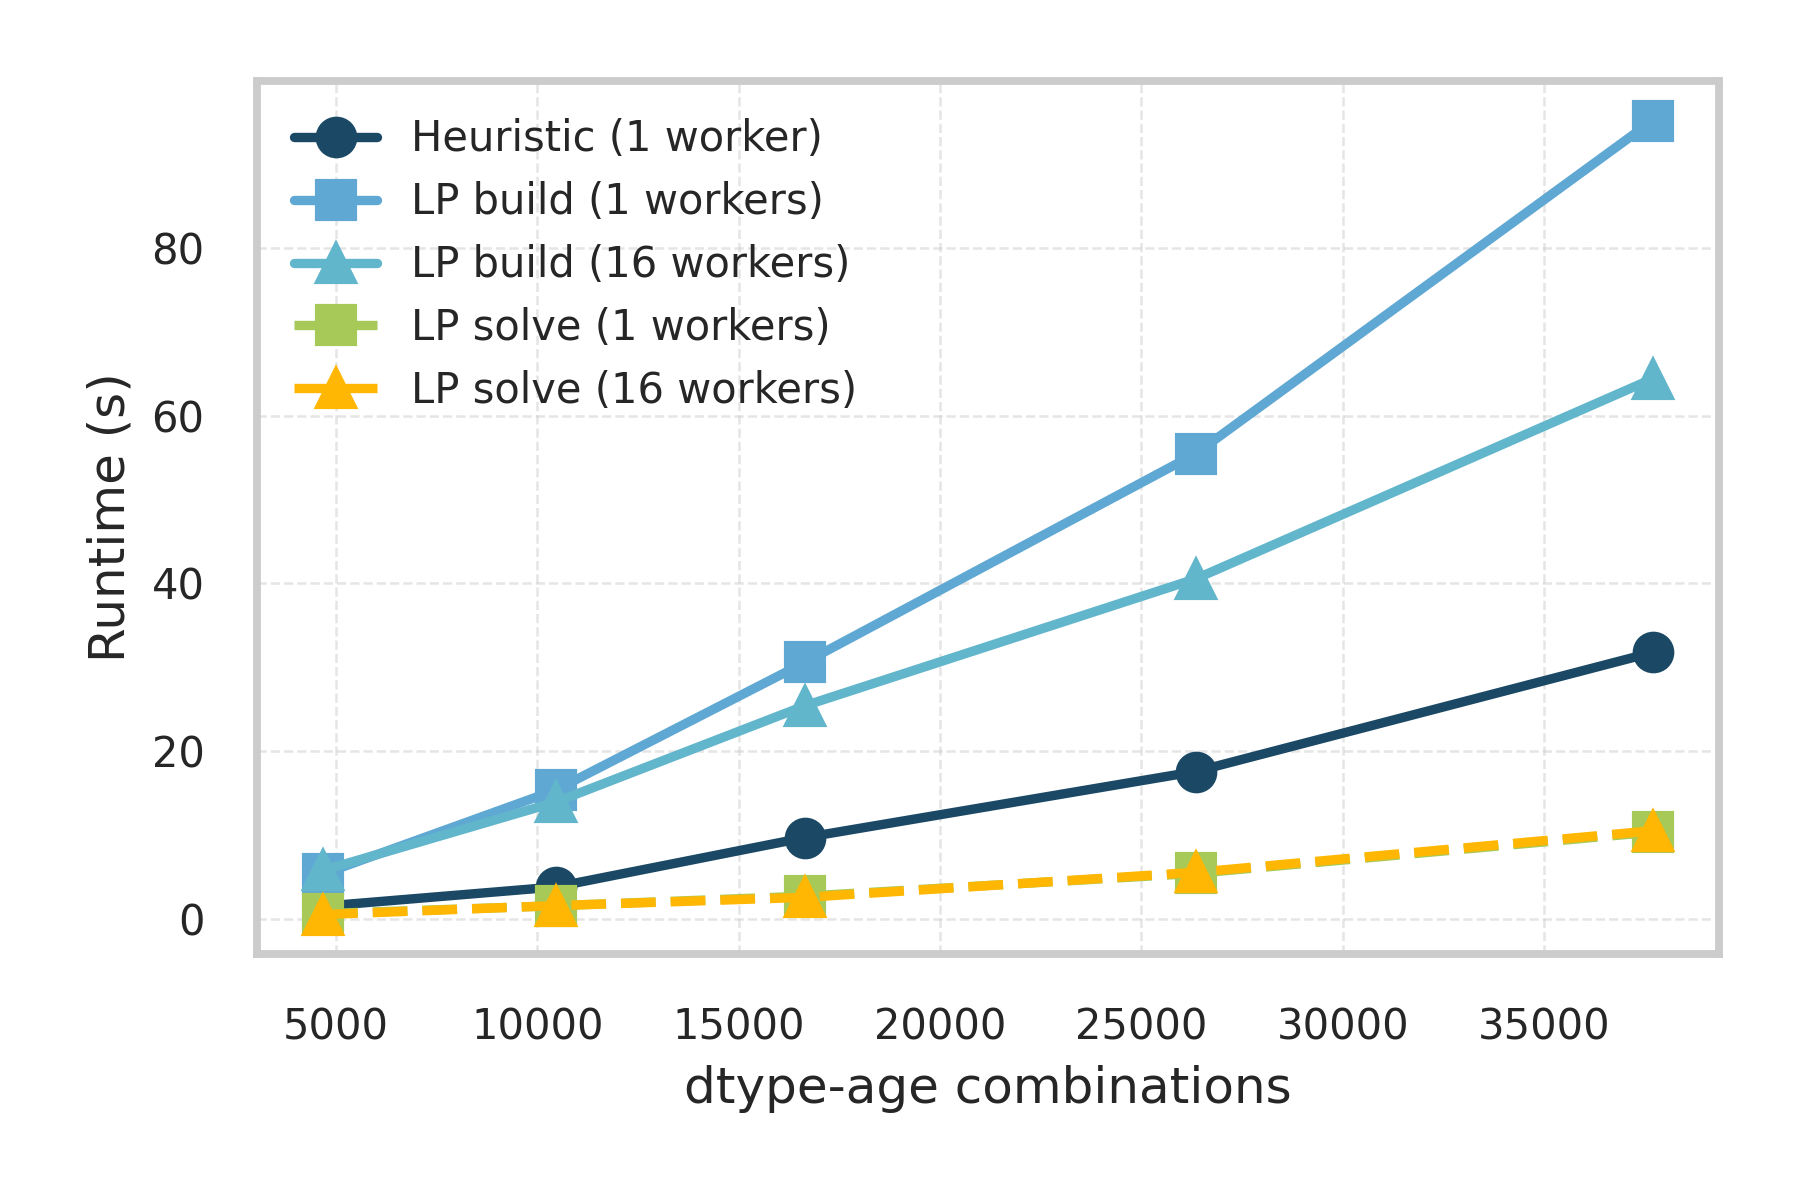
\includegraphics[width=0.85\linewidth]{figs/scaling_schedule_runtime.png}
  \caption{Scheduling runtime versus problem size, measured by the number of development type (dtype) by age combinations ($n_{\text{dtype-age}}$). Heuristic runs are single-worker; LP build/solve lines appear when \texttt{RUN\_LP=1}.}
  \label{fig:scaling_sched}
\end{figure}

\begin{figure}[h]
  \centering
  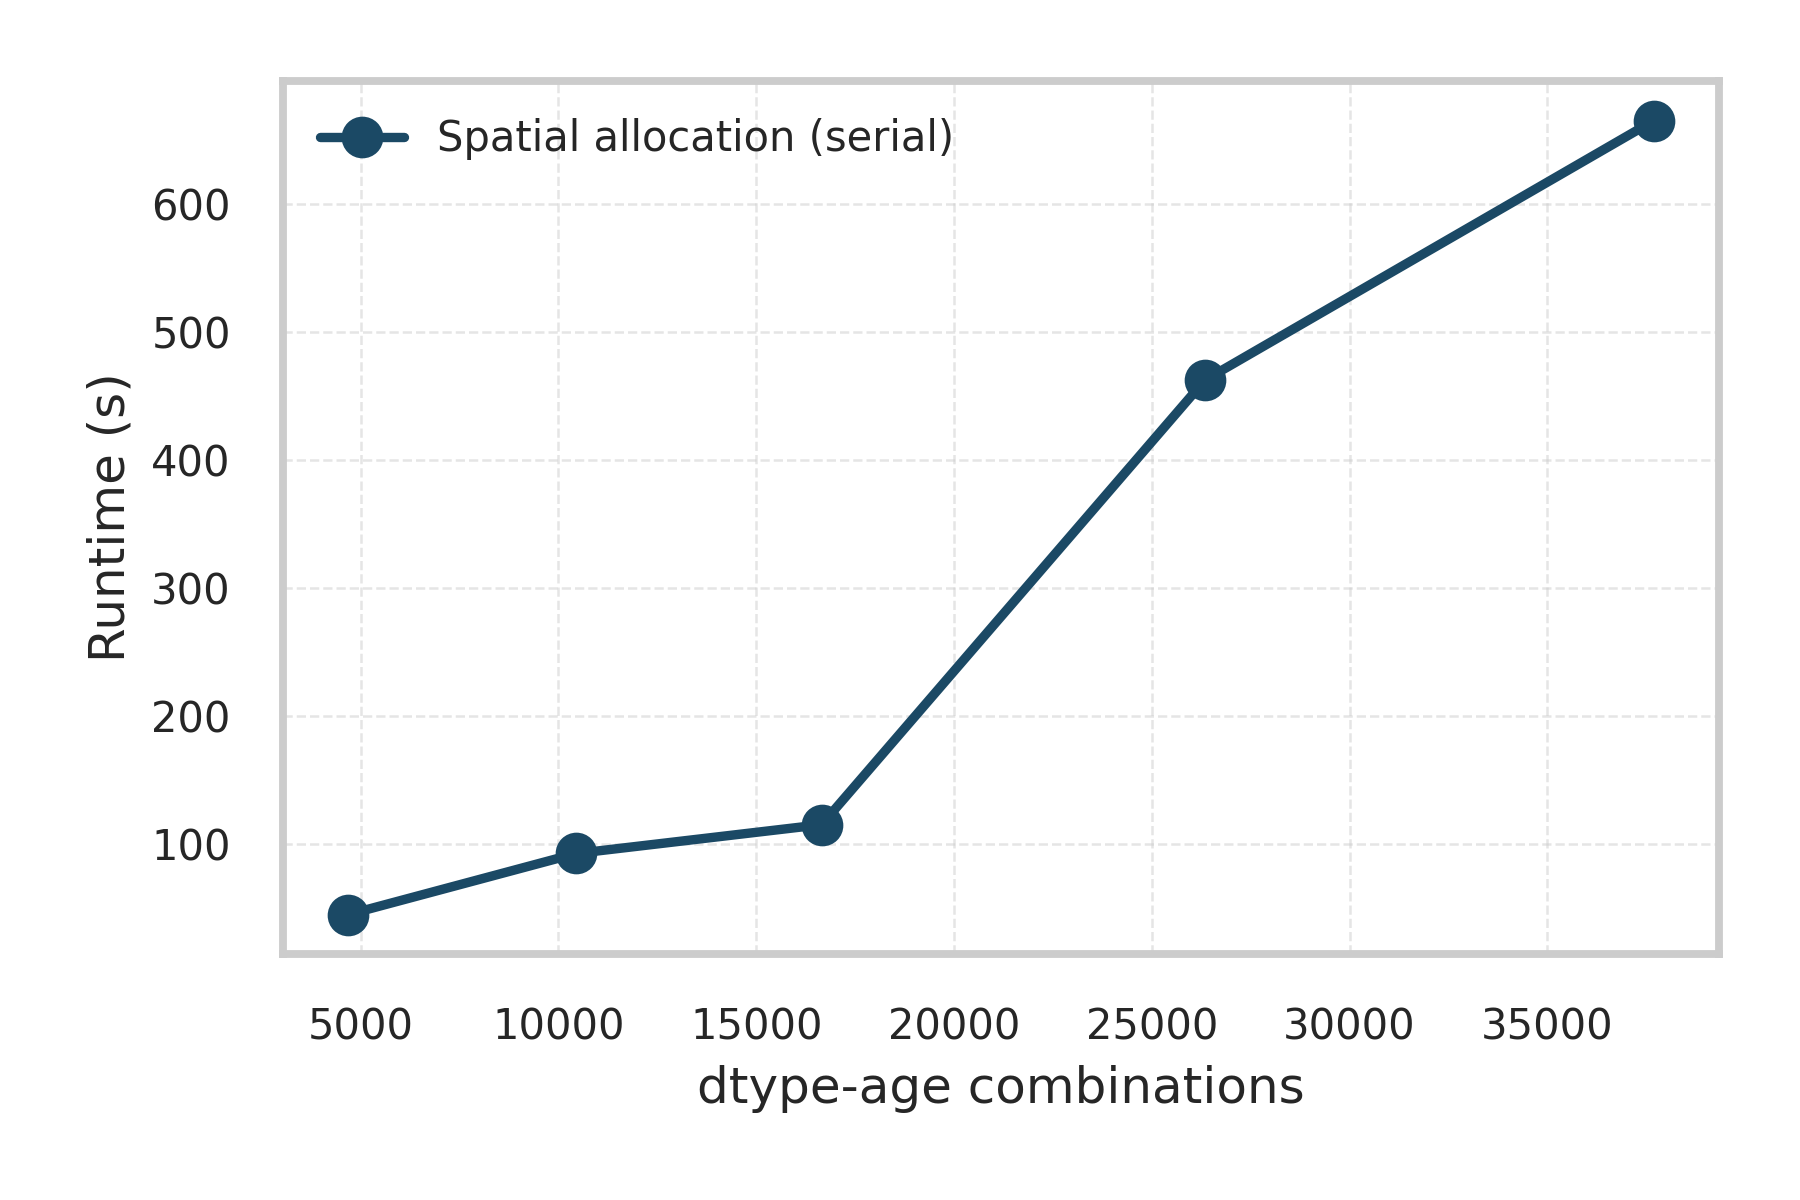
\includegraphics[width=0.85\linewidth]{figs/scaling_spatial_runtime.png}
  \caption{Spatial allocation runtime (serial \texttt{ForestRaster}) versus problem size after applying the heuristic schedule; problem size counts dtype--age combinations ($n_{\text{dtype-age}}$).}
  \label{fig:scaling_spatial}
\end{figure}

\begin{figure}[h]
  \centering
  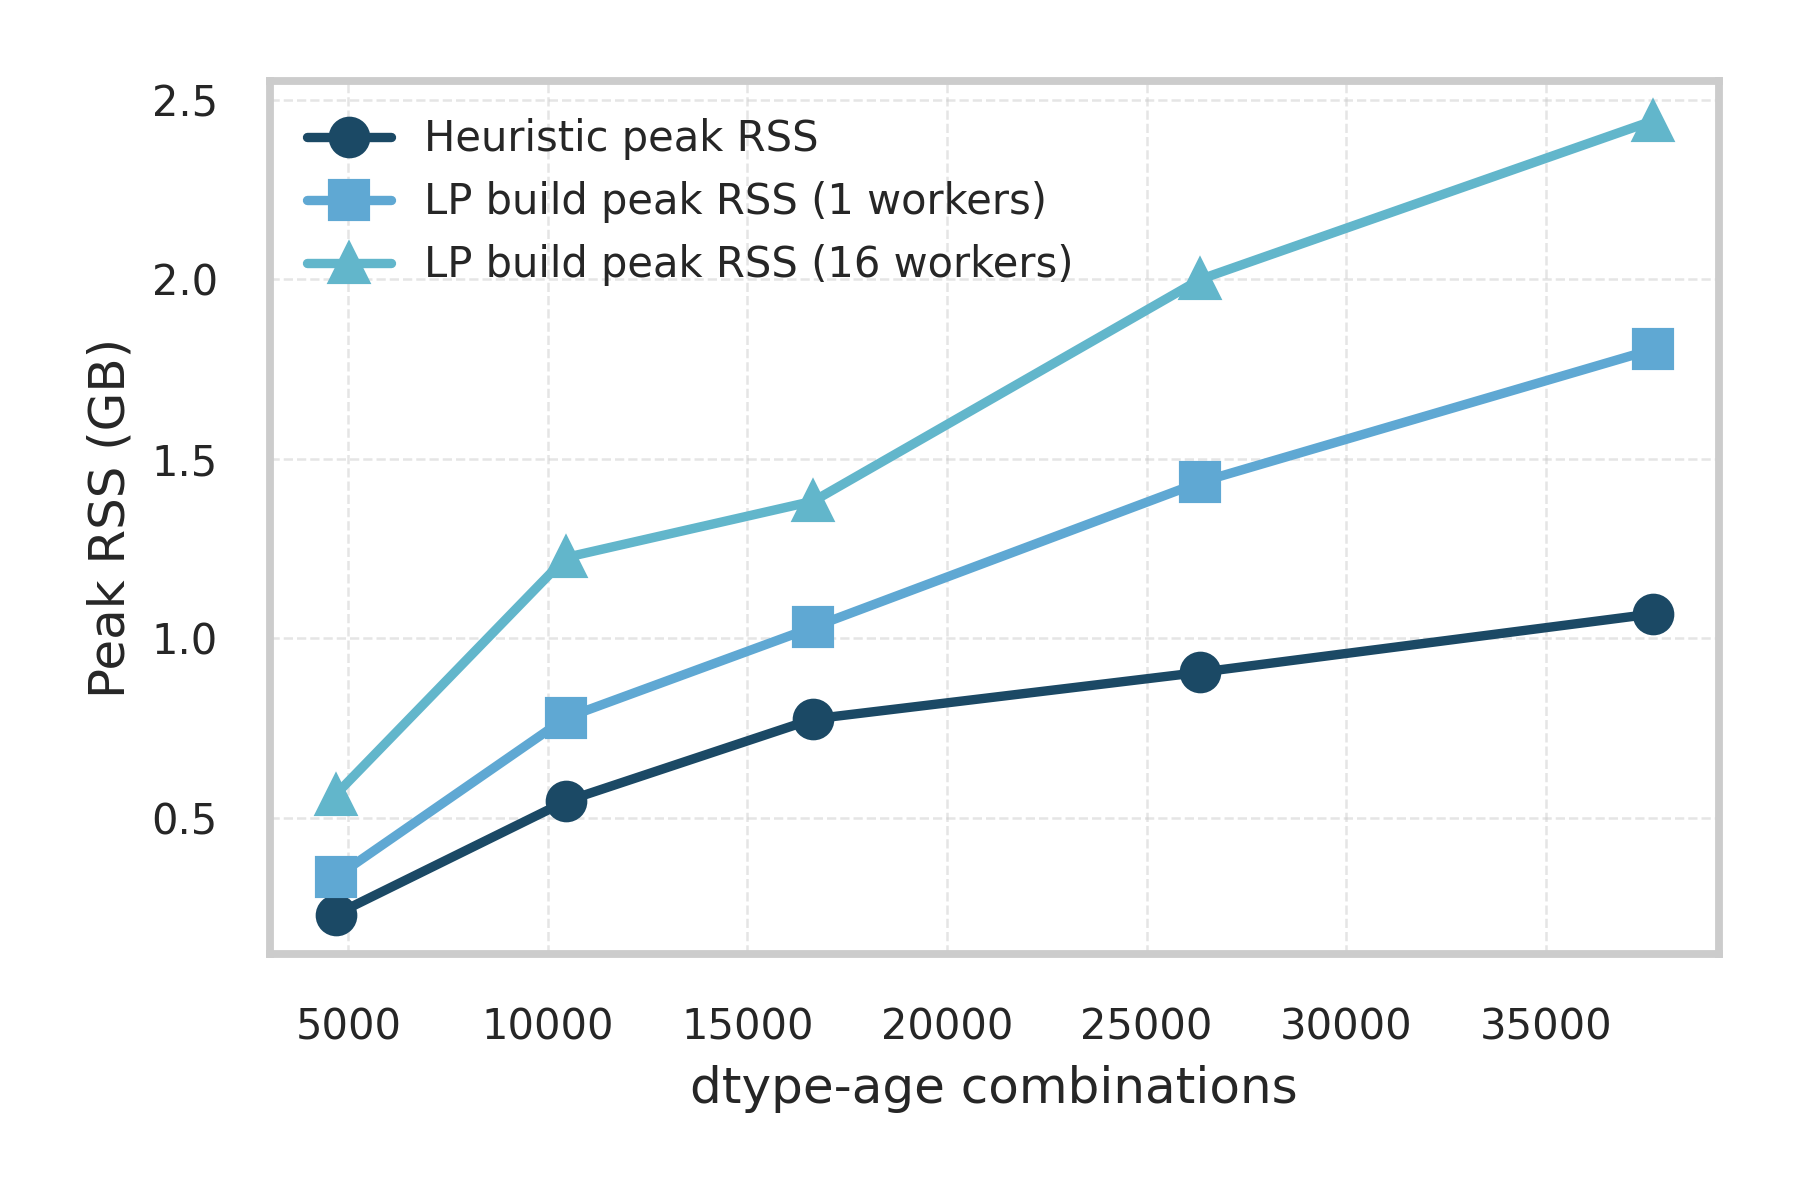
\includegraphics[width=0.85\linewidth]{figs/scaling_peak_mem.png}
  \caption{Peak resident memory for heuristic scheduling (serial) and LP model builds (1 and 16 workers) as problem size increases in terms of dtype--age combinations.}
  \label{fig:scaling_mem}
\end{figure}

\begin{table}[h]
  \centering
  \caption{Peak resident memory during heuristic scheduling and LP model builds on the reference container. $n_{\text{dtype-age}}$ counts development type (dtype) by age combinations; LP measurements report the maximum RSS observed while compiling the Model~I matrix with 1 or 16 workers, while spatial allocation runs serially.}
  \label{tab:scaling_summary}
  \begin{tabular}{lrrrr}
    \toprule
    Combo & $n_{\text{dtype-age}}$ & \shortstack[c]{Heuristic\\peak RSS\\(GB)} & \shortstack[c]{LP peak RSS\\(GB; 1 worker)} & \shortstack[c]{LP peak RSS\\(GB; 16 workers)} \\
    \midrule
    \texttt{tsa08} & 4\,682 & 0.23 & 0.33 & 0.56 \\
    \texttt{tsa08+tsa40} & 10\,453 & 0.52 & 0.78 & 1.22 \\
    \texttt{tsa08+tsa40+tsa41} & 16\,653 & 0.77 & 1.03 & 1.33 \\
    \texttt{tsa08+tsa40+tsa41+tsa24} & 26\,346 & 0.87 & 1.38 & 1.87 \\
    \texttt{tsa08+tsa40+tsa41+tsa24+tsa16} & 37\,691 & 1.07 & 1.81 & 2.51 \\
    \bottomrule
  \end{tabular}
\end{table}


\section{Illustrative use-case demonstrations}
\label{sec:usecase}
We present a two-stage sequential pipeline that schedules harvest in WS3 and then evaluates carbon dynamics using libCBM. The workflow reproduces Example~031 (\texttt{031\_ws3\_libcbm\_sequential-builtin.ipynb}) and is included to ensure reproducibility.

\emph{Study design.} We use the public example dataset \texttt{tsa24\_clipped}. It is intentionally modest so that the full pipeline (scheduling, carbon accounting, and spatial allocation) can be executed and audited on standard hardware, and it mirrors the tutorial dataset distributed with WS3 to keep inputs transparent and reproducible. Inputs are stored as Woodstock-format text files (landscape, areas, yields, actions, transitions) under \path{examples/data/woodstock_model_files_tsa24_clipped} and imported into a \texttt{ForestModel}. We schedule harvest using a self-parameterizing area-control heuristic to produce an aspatial action schedule over a 100-year horizon (10 periods), then export a libCBM Standard Input Table (SIT) to simulate annual carbon stocks and fluxes.

\emph{Data and study area.} The \texttt{tsa24\_clipped} dataset is a clipped subset of a Timber Supply Area inventory used for demonstration. The initial inventory enumerates development types (dtypes) by theme tuples (e.g., analysis unit, species, site), with yield curves for total volume (\texttt{totvol}) and species-volume splits (\texttt{swdvol}, \texttt{hwdvol}). Actions and transitions define operability and state changes (e.g., harvest resets age).

\emph{Model setup and scheduling.} We initialize the model with \texttt{base\_year}=2020, \texttt{horizon}=10, \texttt{period\_length}=10\,y, and \texttt{max\_age}=1000. After importing sections and initializing areas, we add a null action and reset actions. The area-control heuristic proceeds period by period: for each target mask (default: analysis-unit timber-harvesting land base (THLB)), it computes a target area using the area-weighted mean culmination of mean annual increment (CMAI) age and then applies the harvest action to the oldest operable ages within the masked dtype set until the target is met (or inventory is exhausted). This allocation step follows the hierarchical strategic→tactical paradigm described for CRYSTAL-style spatial allocation \citep{jamnick1993spatial} and later operationalized in the Woodstock–Stanley workflow \citep{feunekes1997hierarchical}. In commercial deployments, the spatialization module is now marketed as the Spatial Optimizer (formerly STANLEY) \citep{mistik2019modeling}. The resulting schedule is aspatial, recording treatment area by dtype, age, and period. Utilization is set to 0.85 in the volume expression used for compiled flows. The schedule is compiled and applied to produce period-by-period flows and stocks.

\emph{libCBM coupling and metrics.} We define a disturbance-type mapping for actions (harvest$\to$Clearcut harvesting without salvage; fire$\to$Wildfire) and assign \texttt{last\_pass\_disturbance} per dtype to ensure consistent DOM spin-up. Using \texttt{ForestModel.to\_cbm\_sit} with softwood and hardwood volume names (\texttt{swdvol}, \texttt{hwdvol}), \texttt{admin\_boundary} = \texttt{"British Columbia"}, and \texttt{eco\_boundary} = \texttt{"Montane Cordillera"}, we export the SIT configuration and tables. We then run libCBM for 200 years (\texttt{n\_steps}=200), aggregating annual carbon stocks (biomass, DOM, total ecosystem).

\emph{Outputs.} We report time series of harvested area/volume and growing stock from WS3, and annual carbon stocks from libCBM. Spatial allocation then maps the aspatial schedule onto raster cells using the ForestRaster utility to generate a disturbance footprint while preserving the aspatial totals. The reproduction package generates the figures and tables used below.

The full, deterministic workflow is scripted in \texttt{papers/ems/repro/generate\_case\_study.py}, which produces the flows and carbon stock tables:
\begin{itemize}
  \item \texttt{papers/ems/tables/scenario\_flows.csv}: harvest area, harvest volume, and growing stock by period.
  \item \texttt{papers/ems/tables/annual\_carbon\_stocks.csv}: annual biomass, DOM, and total ecosystem carbon.
\end{itemize}
\begin{table}[h]
\centering
\caption{Sequential demonstration parameters and configuration (WS3 $\to$ libCBM pipeline).}
\begin{tabular}{p{4.2cm}p{9.5cm}}
\toprule
Setting & Value \\
\midrule
Dataset & \texttt{tsa24\_clipped} (Woodstock-format inputs; \texttt{examples/data/woodstock\_model\_files\_tsa24\_clipped}) \\
Base year & 2020 \\
Planning horizon & 10 periods (100 years) \\
Period length & 10 years \\
Max age class & 1000 years \\
Yield names & \texttt{totvol} (total volume), \texttt{swdvol} (softwood), \texttt{hwdvol} (hardwood) \\
Scheduling method & Area-control heuristic (priority-queue, oldest-first); utilization 0.85 \\
Disturbance mapping (CBM) & harvest$\to$Clearcut harvesting without salvage; fire$\to$Wildfire \\
CBM export & \texttt{ForestModel.to\_cbm\_sit} (admin: British Columbia; eco: Montane Cordillera) \\
CBM run length & 200 annual steps \\
Outputs & \texttt{scenario\_flows.csv} (period, harvest\_area\_ha, harvest\_volume\_m3, growing\_stock\_m3); \texttt{annual\_carbon\_stocks.csv} (annual pools) \\
\bottomrule
\end{tabular}
\label{tab:case_params}
\end{table}

Figures~\ref{fig:flows} and~\ref{fig:cbm} show the resulting flows and carbon stocks. The entire pipeline, including the workflow overview (Figure~\ref{fig:workflow_overview}) and the spatial allocation example (Figure~\ref{fig:spatial_allocation}), is reproducible via \path{papers/ems/repro/make_repro.sh}. The libCBM run length (200 years) matches the example but can be adjusted.

Unless stated otherwise, areas are reported in hectares (ha) and volumes in cubic metres (m$^3$).

\begin{figure}[h]
  \centering
  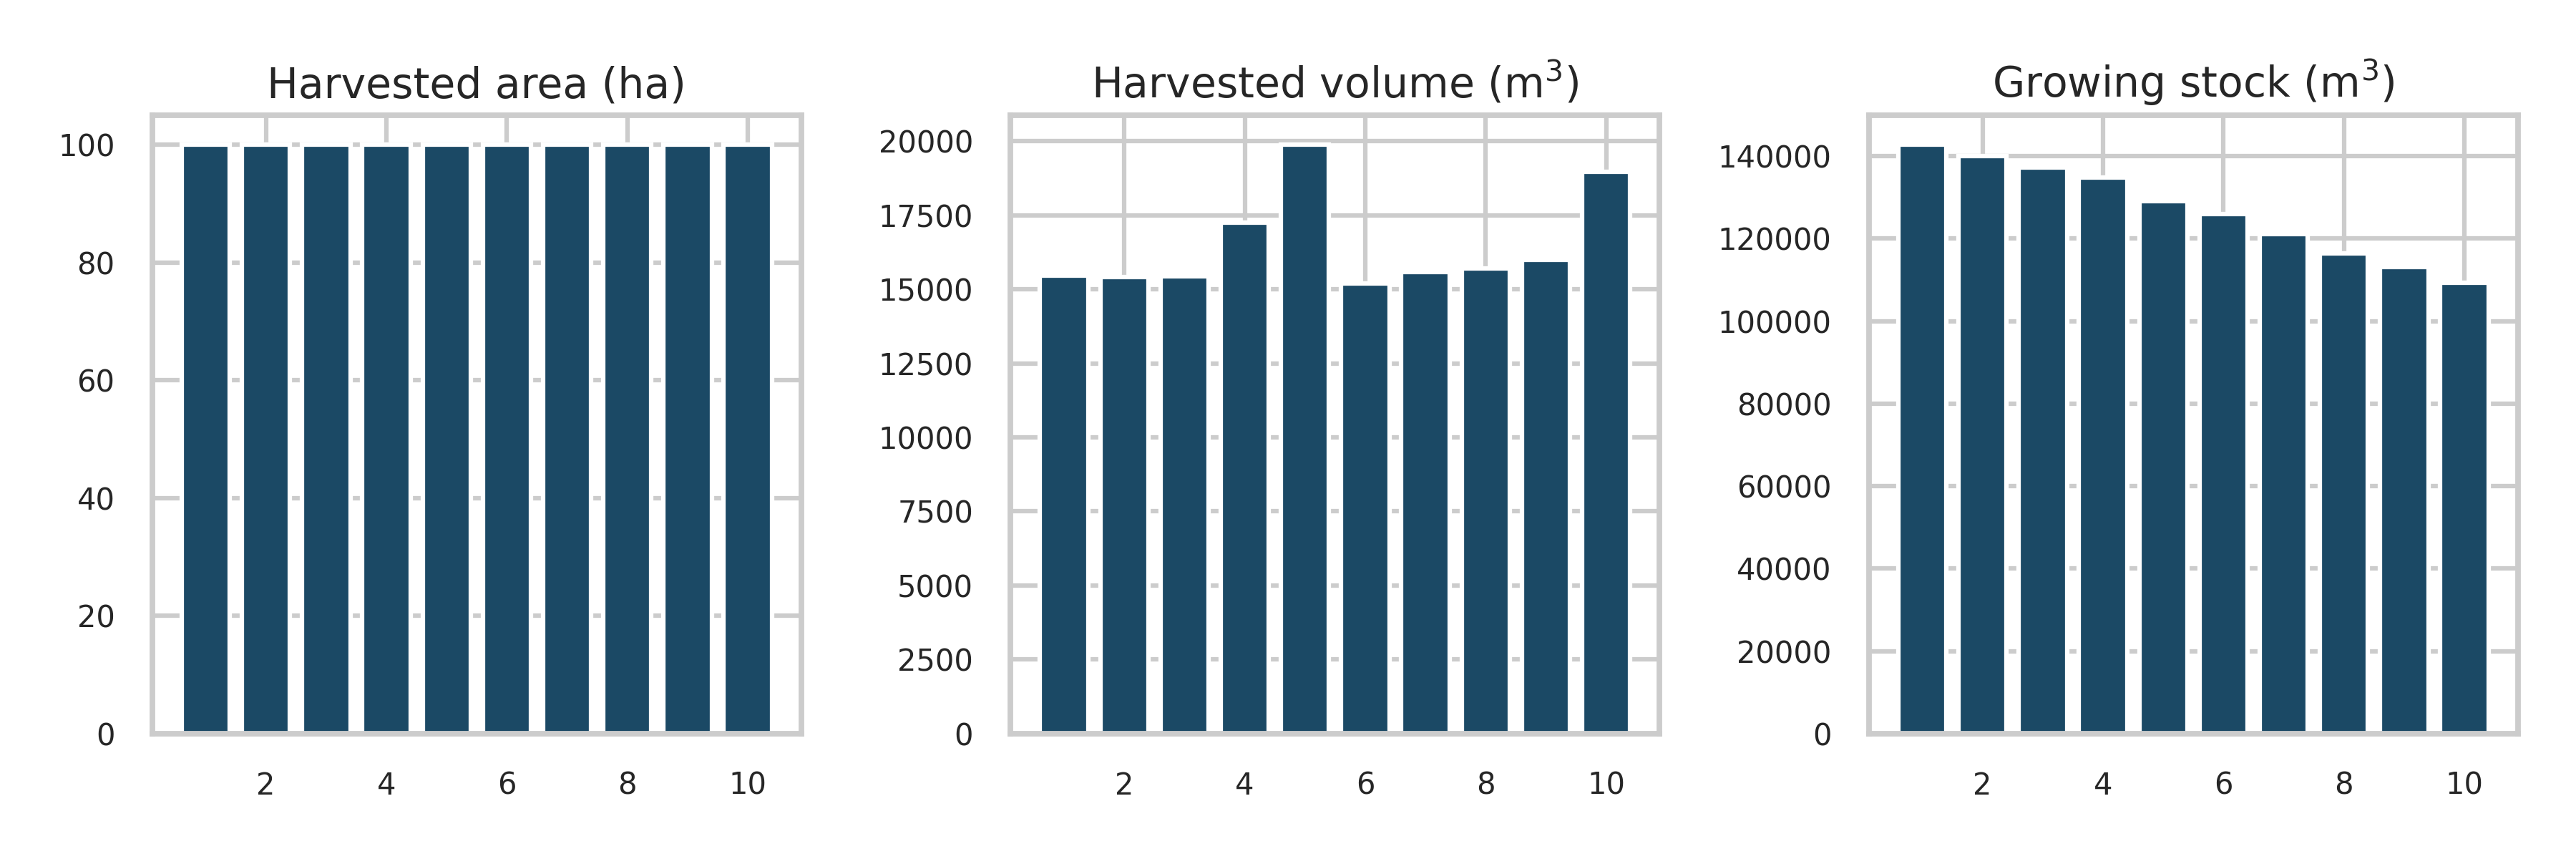
\includegraphics[width=0.95\linewidth]{figs/f4a_harvest_and_stock.png}
  \caption{WS3 results: harvested area, harvested volume (utilization-adjusted), and growing stock over planning periods.}
  \label{fig:flows}
\end{figure}

\begin{figure}[h]
  \centering
  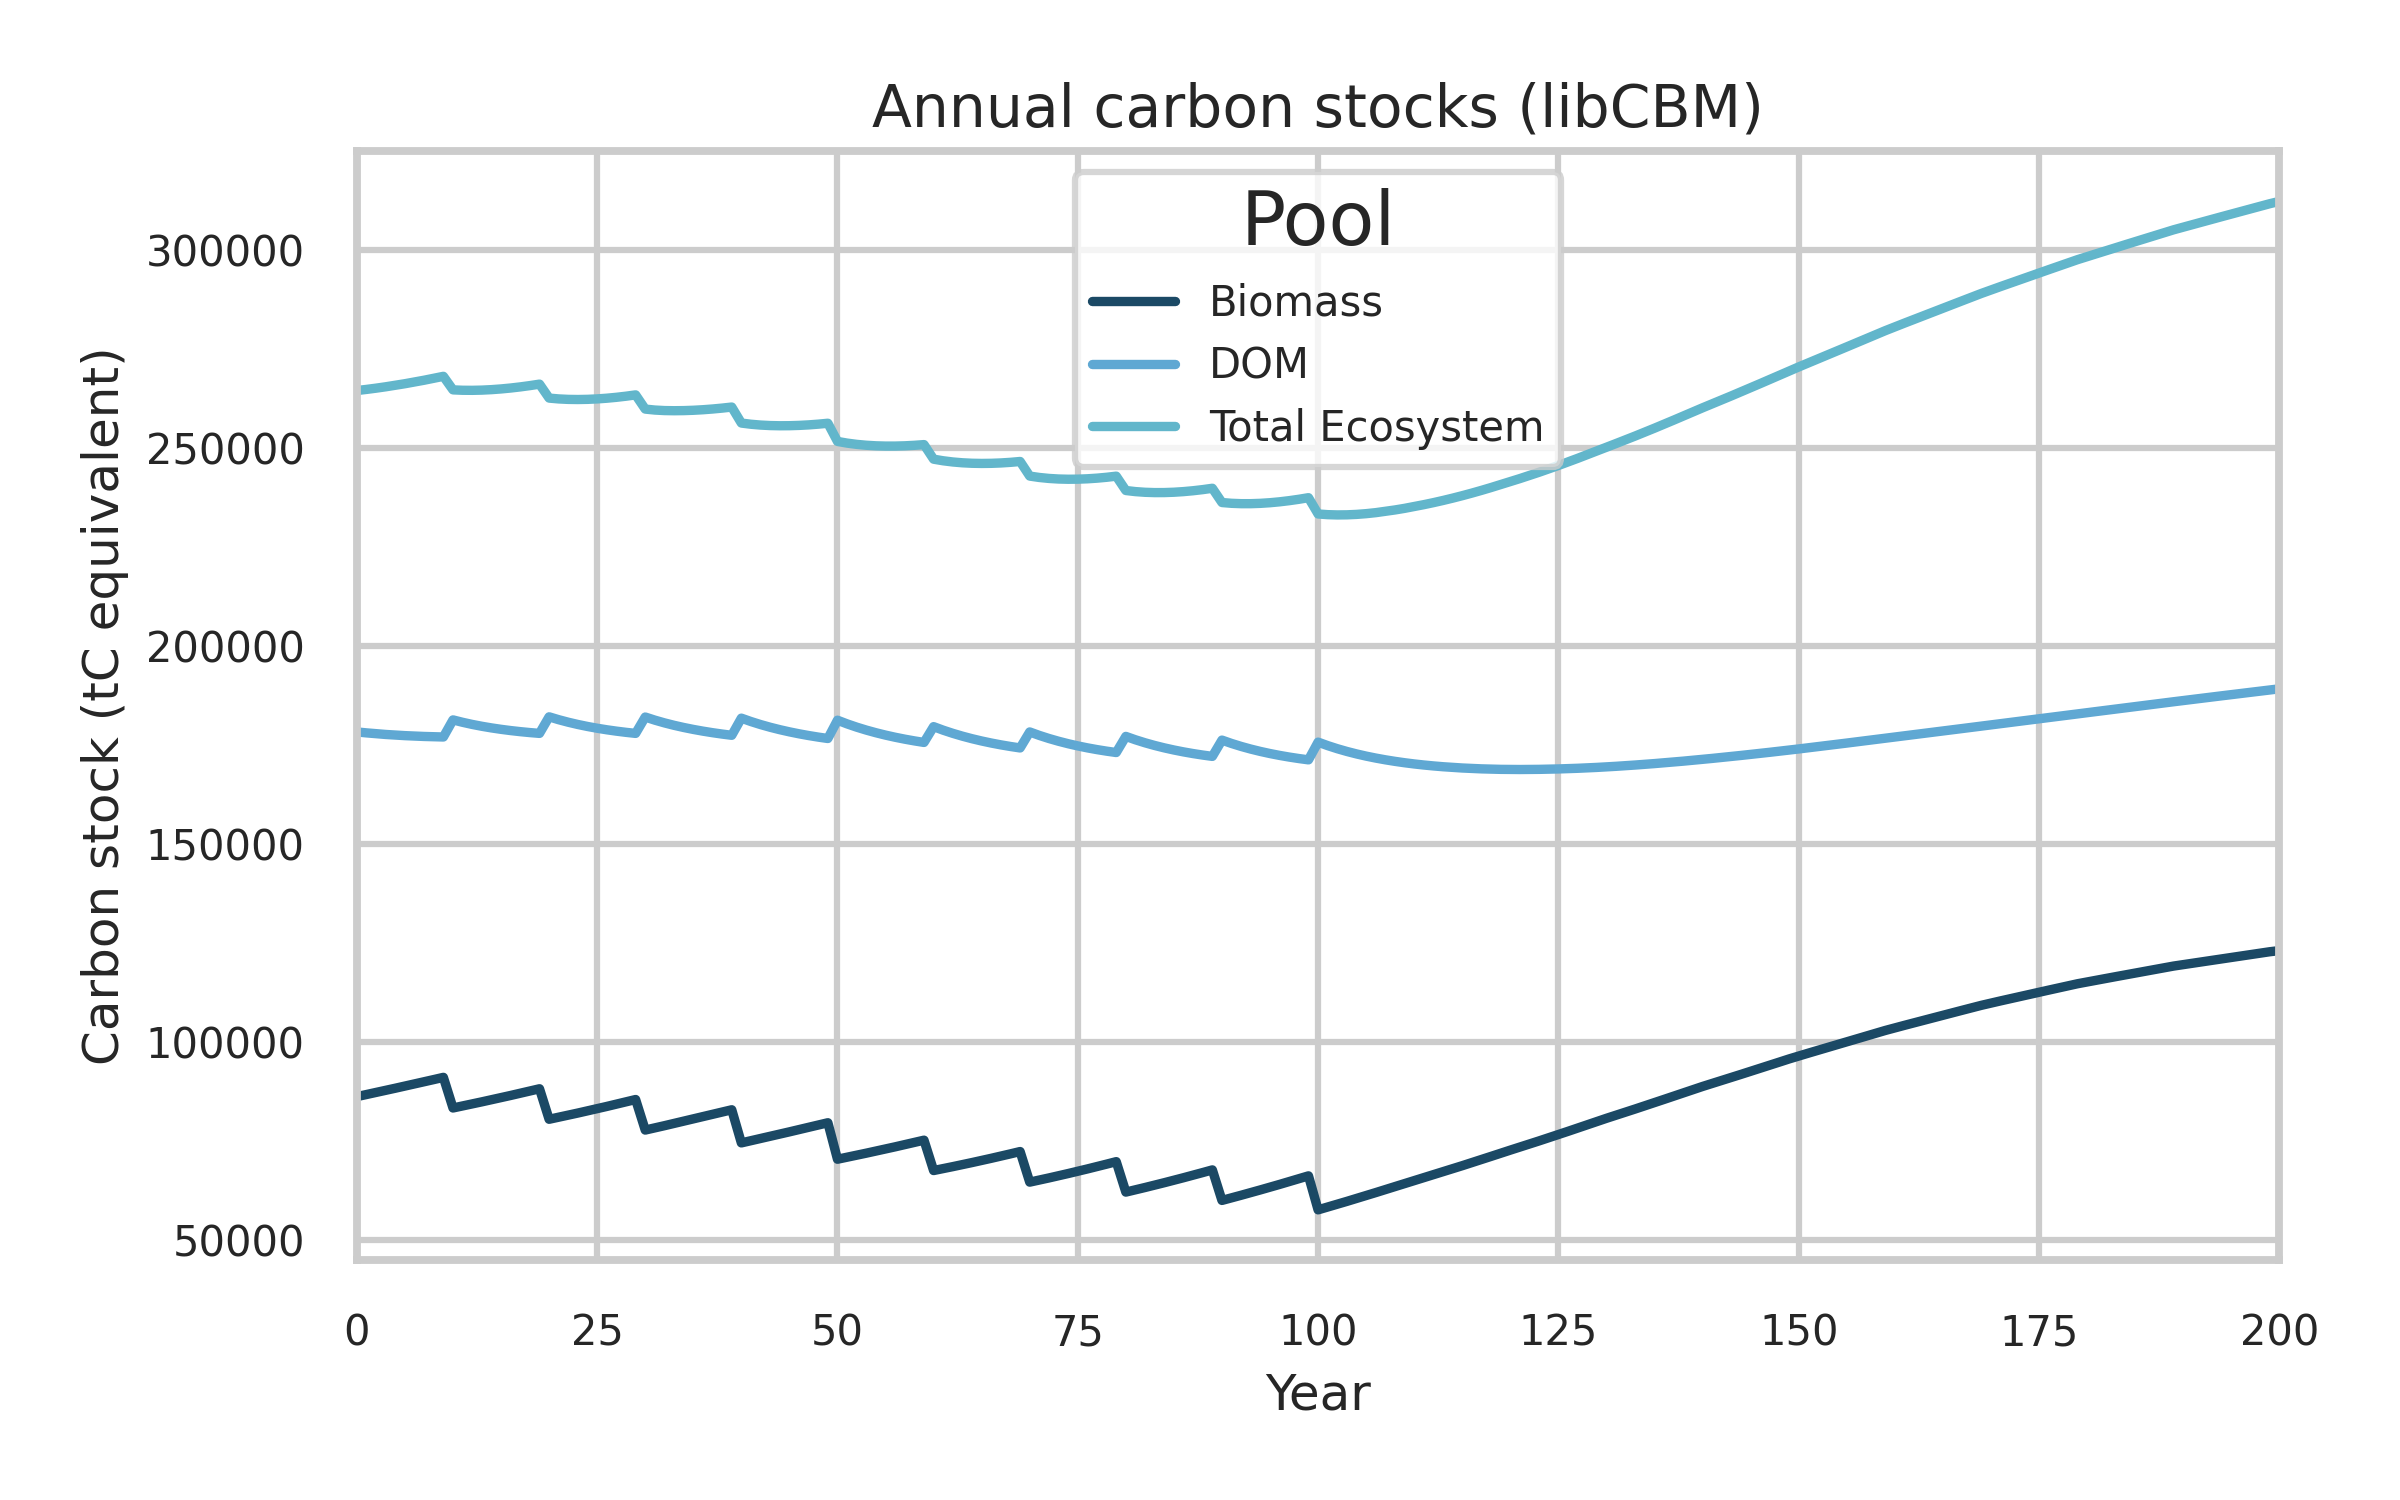
\includegraphics[width=0.95\linewidth]{figs/f4b_carbon_stocks.png}
  \caption{libCBM results: annual carbon stocks (biomass, dead organic matter, total ecosystem) over 200 years.}
  \label{fig:cbm}
\end{figure} 

\emph{Results.} The heuristic scheduler delivers a 10-period harvest plan whose flows stay within \textasciitilde10\% of period means without any explicit even-flow constraint. Harvest area averages 106.8~ha and ranges from 103 to 114~ha, while harvest volume averages 15.3~thousand~m$^3$ and ranges from 14.1--18.5~thousand~m$^3$ (Table~\ref{tab:case_params}; Figure~\ref{fig:flows}). Growing stock declines smoothly from 135~thousand to 82~thousand~m$^3$ (consistent with the 0.85 utilization factor), reflecting the state trajectory exported to libCBM. In the carbon stage, libCBM aggregates show biomass pools increasing from $2.7\times10^5$~tC to $3.1\times10^5$~tC over 200 years, while DOM remains within $1.7$--$1.9\times10^5$~tC, yielding a total ecosystem carbon gain of 42~ktC (Figure~\ref{fig:cbm}). These values are illustrative; the key contribution is the deterministic, auditable pipeline that connects scheduling outputs to carbon accounting and spatial allocation with byte-identical outputs. The summary tables \texttt{scenario\_flows.csv} and \texttt{annual\_carbon\_stocks.csv} (\texttt{papers/ems/tables}) retain raw outputs for external verification.

\emph{Reproducibility.} This demonstration is intended to be transparent and portable. All input data reside in \path{examples/data/woodstock_model_files_tsa24_clipped}. The spatial allocation step produces the raster-based harvest allocation shown in Figure~\ref{fig:spatial_allocation}, derived directly from the aspatial schedule via the ForestRaster utility. The folder \path{papers/ems/repro} contains \path{make_repro.sh}, which provisions a clean virtual environment, installs pinned dependencies (including the optional libCBM extra via \texttt{pip install ws3[cbm]}), and runs deterministic scripts that regenerate Figures~\ref{fig:workflow_overview}--\ref{fig:cbm} and the accompanying CSV tables. Outputs are byte-identical on the reference container and stable under the pinned dependencies. The exact environment is preserved in the Zenodo-archived release.

\subsection*{Broader example library and carbon-aware optimization}
Beyond the sequential carbon accounting demonstration, WS3 includes executable notebooks that serve as tutorials and validation exercises, ranging from synthetic cases to policy-oriented analyses. Example~040 implements the Neilson hack and compares aggregated WS3 carbon indicators with libCBM in a no-disturbance scenario. Example~041 illustrates carbon-aware optimization by embedding carbon prices/constraints in the LP and evaluating schedules with \texttt{libcbm\_py}.
%A public, end-to-end use-case demonstration exploring carbon-aware scheduling in a stylized British Columbia landscape is available in the repository by Yan (MSc), including scenario automation, sensitivity analysis, and reproducible outputs \citep{yan2025mathematical, yan_repo}.

\begin{figure}[h]
  \centering
  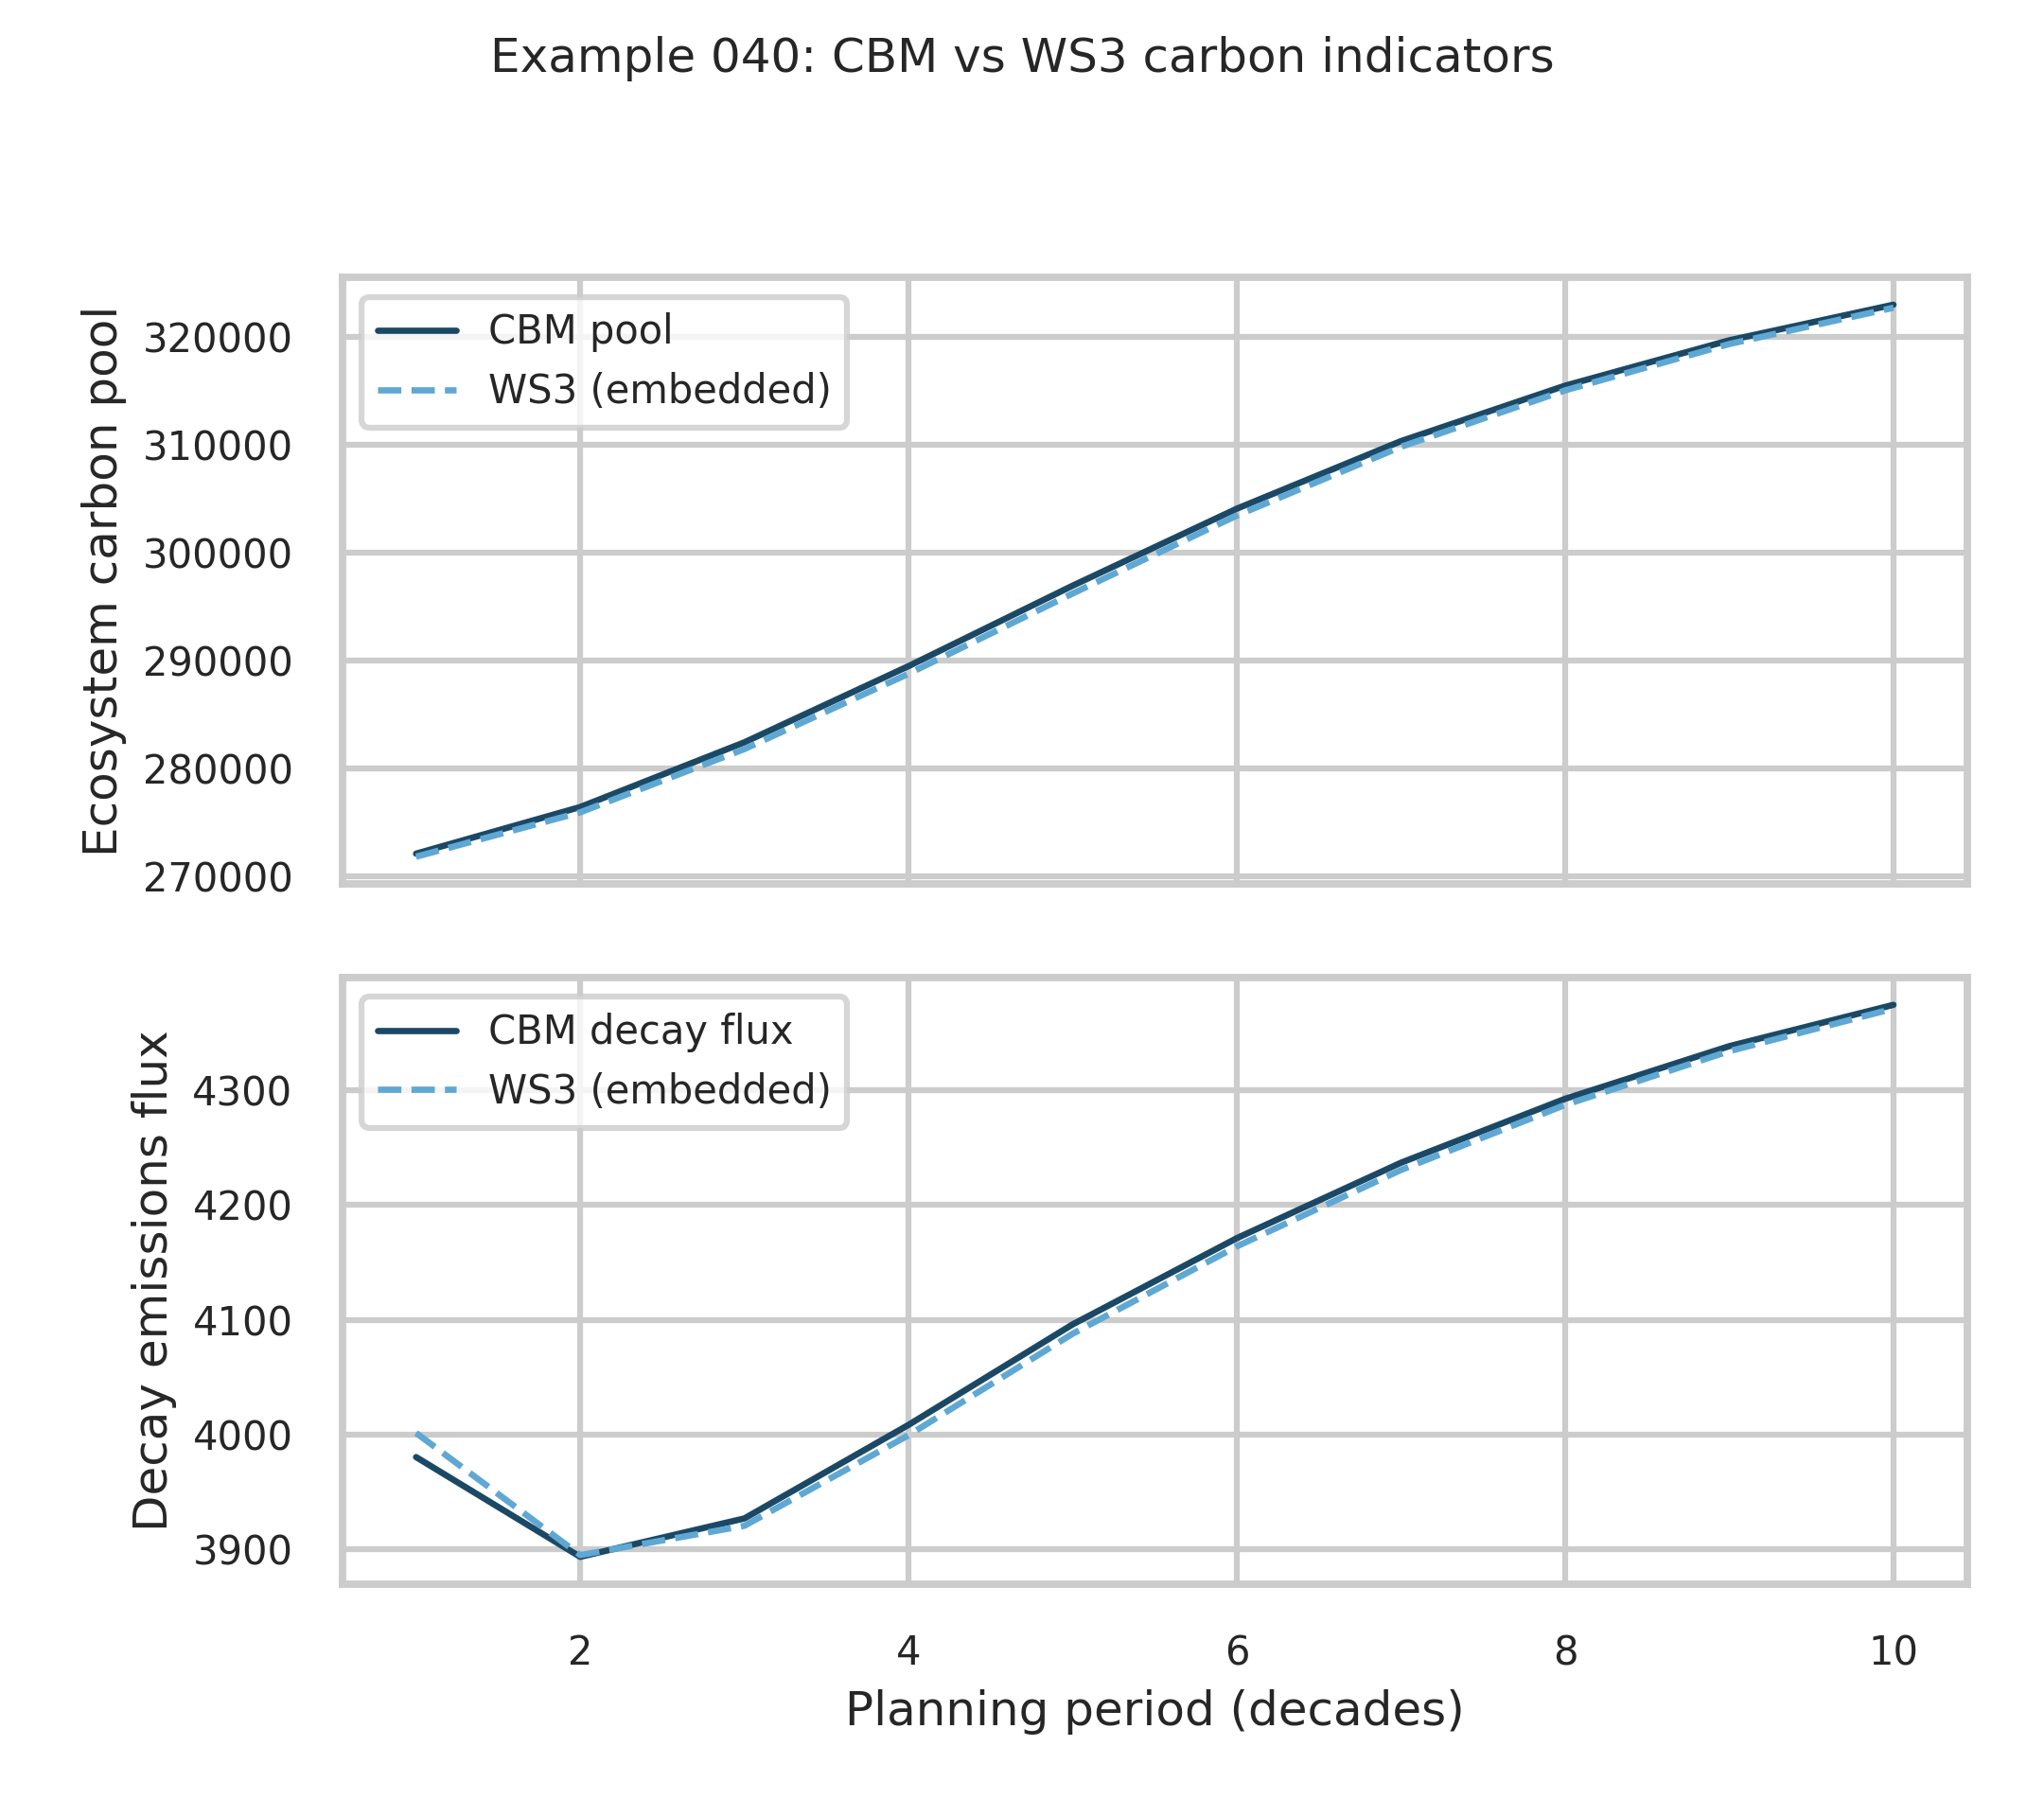
\includegraphics[width=0.95\linewidth]{figs/f5_neilsonhack_compare.png}
\caption{Neilson-hack demonstration (Example~040): comparison of libCBM (solid) and WS3-embedded (dashed) carbon indicators after bootstrapping pools/fluxes into WS3 as yield curves. Top: ecosystem carbon pools; bottom: aggregate decay emissions flux. In a no-disturbance scenario, the aggregated indicators match closely; with harvesting, flux gaps reflect known limitations of the Neilson hack due to CBM DOM spin-up assumptions mapping time to age (Figure~\ref{fig:neilsonhack}).}
  \label{fig:neilsonhack}
\end{figure}

\section{Impact and reusability}

WS3 has been used in research on bioenergy \citep{cantegril2019bioenergy}, value-creation potential and supply modeling \citep{paradis2018retro, paradis2018estimating}, and climate impact assessment \citep{smyth2020climate, ke2024climate, yan2025mathematical}. It integrates with the SpaDES ecosystem for spatial simulation \citep{spades} and has been deployed as a backend in decision-support applications. The MIT license, modular API, and PyPI distribution support reuse across jurisdictions.

\paragraph{Major use cases (2015--2025)}
\begin{itemize}
  \item Strategic wood supply and bioenergy planning in mixed-wood forests: optimization and scenario analysis of value-creation options \citep{cantegril2019bioenergy}.
  \item Hybrid simulation--optimization for value indicators and model retrofitting: methods and transfer to production-style analyses \citep{paradis2018retro, paradis2018estimating}.
  \item Climate mitigation and carbon-aware planning in British Columbia: sequential WS3$\to$libCBM pipelines and optimization under policy constraints; graduate theses and applied demonstrations \citep{ke2024climate, yan2025mathematical, yan_repo}.
  \item Decision-support prototypes for nature-based solutions: avoided fire and avoided harvest workflows (Examples~050/060) with net-emission indicators derived from libCBM.
  \item Integration with spatial simulation: \texttt{spades\_ws3} module bridging WS3 with SpaDES for disturbance and landscape dynamics studies \citep{spades, spades_ws3}.
  \item Application backends: WS3 used in web-based decision-support systems (e.g., \texttt{ecotrust-dss}) for scenario configuration and reporting \citep{ecotrust-dss}.
  \item Ongoing initiatives: CCCANDiES (integrated carbon and ecosystem services; in progress) and mining-sector nature-based solutions \citep{ghasemi2025decarbonization}.
\end{itemize}

Interoperability is supported through tabular/text inputs, raster outputs, and the libCBM linkage, enabling WS3 to integrate with existing analytical pipelines. The reproduction package, unit tests, and continuous integration (CI) pipelines facilitate method transfer and support open scientific practices \citep{hampton2015tao, lowndes2017path}. The architecture is general and has been applied to studies of sustainable yield, carbon accounting, biodiversity, and policy trade-offs \citep{boisvenue2022managing}.

\paragraph{Reusability features}
\begin{itemize}
  \item Openness and packaging: MIT license, PyPI distribution, versioned releases archived on Zenodo \citep{ws3_zenodo2025}; complete examples and tutorials.
  \item Interoperability: Woodstock-format import for legacy/industry pipelines; libCBM SIT export for carbon; standard geospatial formats (GeoTIFF, shapefiles).
  \item Reproducibility: deterministic reproduction package (\path{papers/ems/repro}) that regenerates all figures and tables; continuous integration (CI) pipelines run tests and validate examples.
  \item Extensibility: modular API for adding outputs/constraints and new scheduling logic (heuristic or LP-based); solver-flexible (HiGHS by default; Gurobi optional).
  \item Integration pathways: SpaDES ecosystem via \texttt{spades\_ws3}; backend for decision-support applications and web services.
  \item Education and onboarding: progressive example notebooks (from \texttt{010} to \texttt{060}) facilitate training and method transfer.
\end{itemize}

Example~040 demonstrates a stand-level optimization workflow with explicit integration of carbon dynamics using \texttt{libcbm\_py}. The workflow shows how WS3’s optimization layer and libCBM coupling can support carbon-aware planning experiments while leaving the precise objective formulation to the user.

\section{Comparison to alternatives}

\begin{table}[h]
  \centering
  \caption{Comparison of WS3 with selected tools.}
  \begingroup
  \setlength{\tabcolsep}{3pt}
  \renewcommand{\arraystretch}{0.92}
  \footnotesize
  \begin{tabular}{p{2.4cm}p{2.1cm}p{1.5cm}p{2.0cm}p{2.0cm}p{1.9cm}p{1.9cm}}
  \toprule
  Tool & Scope & License & Optimization & Spatial & Carbon & Region \\
  \midrule
  WS3 & Landscape & Open (MIT) & Built-in (PuLP; optional Gurobi) & Hybrid aspatial-to-raster & Built-in libCBM linkage & General \\
  Woodstock & Landscape & Proprietary & Built-in & Extensions; connectors & External integrations & General \\
  Patchworks & Landscape & Proprietary & Built-in & Spatial planning emphasis & External integrations & General \\
  SpaDES & Simulation framework & Open & External packages & Fully spatial (agent-based, raster) & Via modules & General \\
  Heureka & Landscape & Restricted (mixed) & Built-in & Spatial capabilities & External integrations & EU-focused \\
  JLP (MELA) & Landscape & Restricted (legacy) & Built-in & Spatial extensions & External integrations & Finland-focused \\
  \bottomrule
  \end{tabular}
  \endgroup
\end{table}

\paragraph{Parity with Woodstock}
To demonstrate that WS3 implements standard inventory accounting correctly, we report a parity check against a reference Woodstock run using the same toy dataset and an identical action schedule. This test is a transparent, reproducible illustration rather than an exhaustive proof of equivalence. The accompanying CSV artifact \path{papers/ems/tables/woodstock_parity.csv} provides total harvest area, harvest volume, and growing stock, along with WS3-relative percent differences (computed as $100\,(\mathrm{WS3{-}Woodstock})/\mathrm{Woodstock}$). For transparency, period-wise parity summaries for harvest area and volume can be regenerated via the reproduction scripts and are included in the reproduction package (Figure~\ref{fig:sup_parity_periods}). Exact or near-exact agreement is expected given identical inputs.

\begin{table}[h]
  \centering
  \caption{WS3 vs. Woodstock parity on the toy dataset (identical schedule). Values are loaded from the accompanying CSV artifact.}
  \label{tab:woodstock_parity}
  \footnotesize
  \begin{tabular}{lrrr}
    \toprule
    Metric & WS3 & Woodstock & WS3 vs Woodstock (\%) \\
    \midrule
    Total harvest area (ha) & 1,000.00 & 1,000.00 & 0.00 \\
    Total harvest volume (m$^3$) & 164,838.08 & 164,838.08 & 0.00 \\
    Total growing stock (m$^3$) & 1,269,692.15 & 1,269,692.15 & 0.00 \\
    \bottomrule
  \end{tabular}
\end{table}

\begin{figure}[htbp]
  \centering
  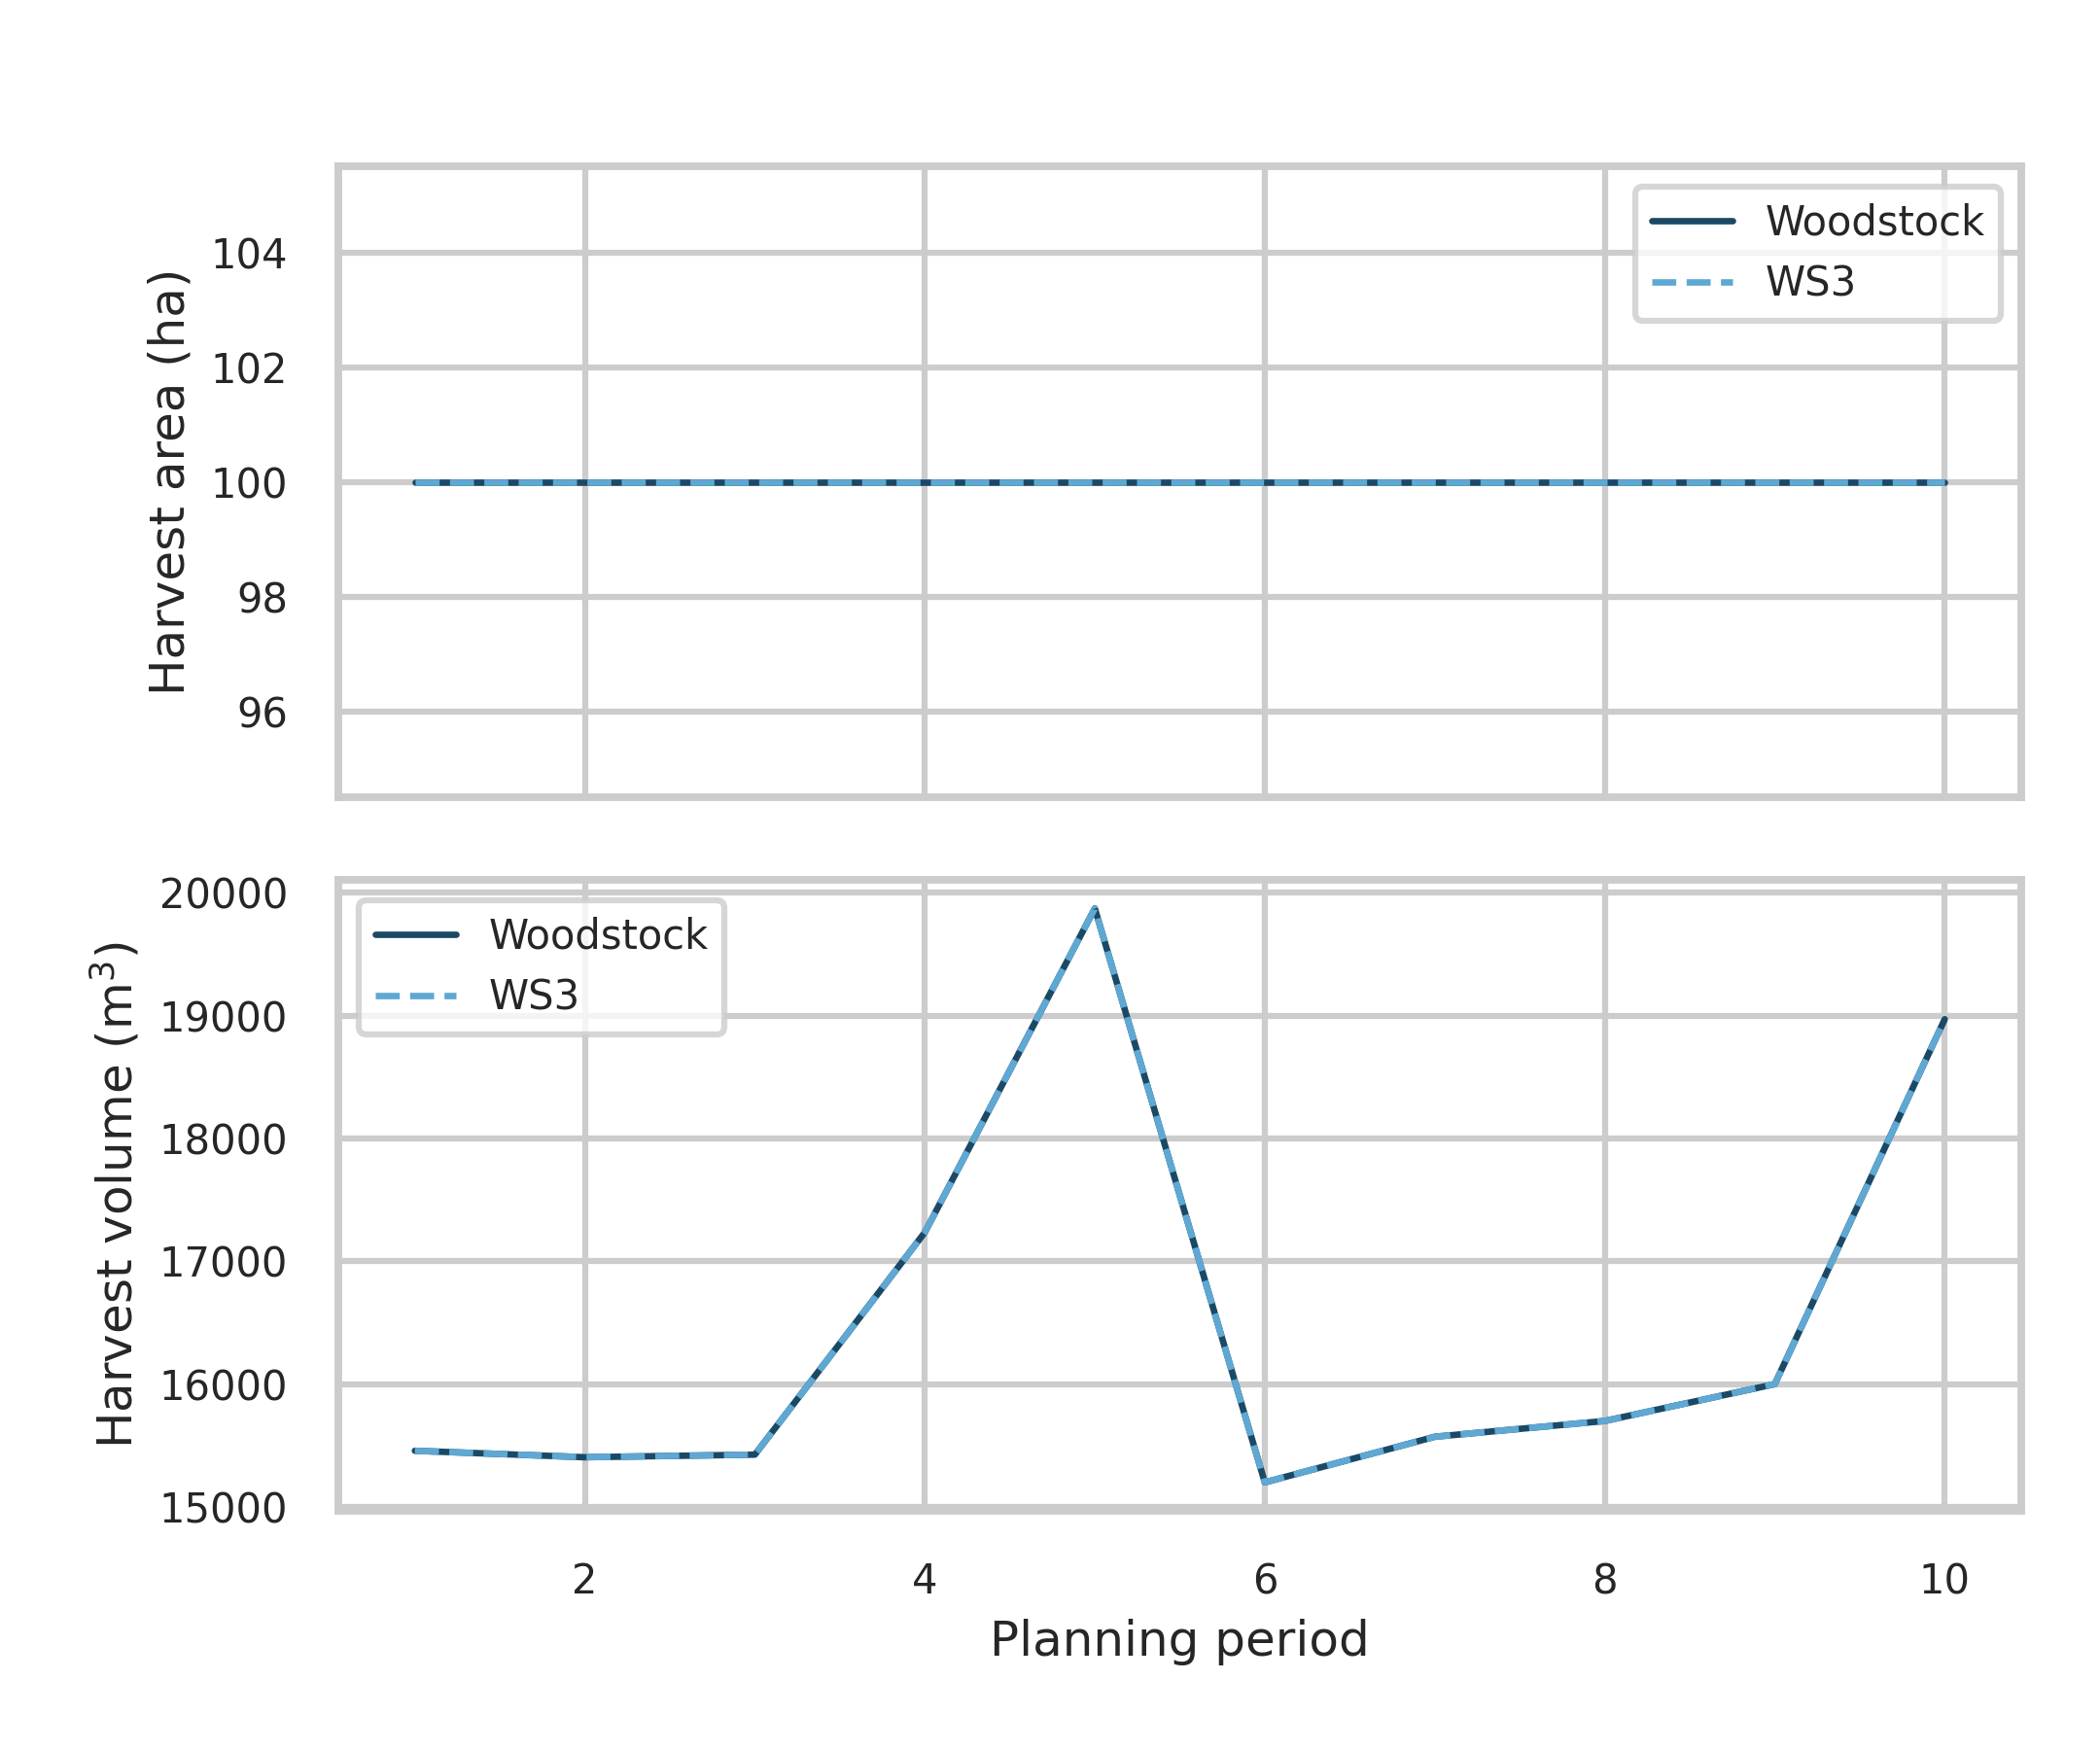
\includegraphics[width=0.95\linewidth]{figs/sup_parity_periods.png}
  \caption{Period-wise parity of harvested area and harvested volume between WS3 and Woodstock on the toy dataset (identical schedule). Values are loaded from the accompanying CSV artifact.}
  \label{fig:sup_parity_periods}
\end{figure}

\noindent
WS3 provides an open Python API, a documented libCBM integration, and a hybrid spatial/aspatial workflow intended for reproducible analyses. It is a framework rather than a GUI decision-support suite; spatial adjacency, opening-size constraints, and road-network planning are outside its scope. Woodstock, Patchworks, Heureka, and JLP target landscape-scale planning with varying degrees of spatial explicitness and availability \citep{remsoft-woodstock, patchworks, spades, heureka, jlp_mela}.

\paragraph{Comparison narrative}
Proprietary landscape systems such as Woodstock and Patchworks offer mature optimization and spatial planning capabilities, including native support for adjacency and block constraints, but their licensing and closed codebases can limit transparent methods development and reproducibility at scale. SpaDES is an open simulation framework oriented to spatial processes and agent-based dynamics; it does not natively provide a solver-backed harvest scheduling layer but can interoperate with WS3 via \texttt{spades\_ws3} for hybrid workflows. Heureka and JLP are landscape-oriented and include optimization, yet are region-specific or legacy-maintained, which constrains adoption beyond their primary jurisdictions.

Carbon-aware planning and optimization have an active literature that couples timber supply models with carbon accounting and evaluates mitigation trade-offs under alternative schedules and policies. Early integrations such as CO2Fix paired with timber supply modeling illustrate carbon-informed planning workflows \citep{neilson2006co2fix}. More recent sector and landscape studies quantify mitigation potential and carbon capacities under harvest scenarios \citep{smyth2020climate, boisvenue2022managing}, and graduate theses in British Columbia explicitly evaluate climate objectives in forest planning optimization contexts \citep{ke2024climate, yan2025mathematical}. WS3 provides a reproducible, open framework for constructing these workflows while keeping the scheduling engine transparent and auditable.

WS3 integrates: (i) a solver-flexible, path-based Model~I LP generator embedded in an open forest estate API; (ii) a documented linkage to libCBM for carbon stocks and fluxes; and (iii) a hybrid spatial/aspatial pipeline with standard geospatial I/O. This design supports reproducible workflows in notebooks and scripts and integrates with larger research and decision-support ecosystems. Where spatially explicit optimization is required, WS3 can provide schedules and carbon accounting inputs to specialized spatial tools; carbon-related objectives or constraints can be added when users supply coefficients, but they are not required for the core workflow demonstrated here.

\section{Discussion}
WS3 is intended as an open, reproducible alternative to proprietary forest estate planning systems. Its contribution is primarily informatics: a transparent, scriptable workflow that integrates scheduling, carbon accounting, and spatial reporting, rather than a new optimization formulation.

\subsection{Scope and limitations}
WS3 focuses on deterministic, aspatial forest estate formulations. It does not attempt to represent stochastic risk, uncertainty propagation, machine learning forecasting, or fully spatial optimization; those are handled through scenario ensembles or specialized tools rather than within the core framework. The Model~I LP implementation is well suited to even-flow policies, policy bounds, and value maximization problems, yet it inherits classic limitations of the formulation: stochastic or endogenous disturbances cannot be represented faithfully without leaving linearity, and non-linear objectives or constraints require either linearization or external wrappers. In practice, we use the heuristic scheduler to run disturbance realizations or sensitivity analyses when scenario logic demands it, and reserve the LP for static policy experiments.

Spatial representation is provided through a post hoc raster allocation step that respects operability and transitions but does not enforce spatial adjacency, road-building, or block-shape constraints. Those dynamics fall outside the scope of WS3. Users requiring spatial optimization should therefore treat WS3 as a scheduling and accounting engine that feeds specialized spatial tools.

In this manuscript, carbon accounting is applied post hoc to schedules produced by the LP or heuristic workflows. The framework can be extended to incorporate carbon-related objectives or constraints when users supply the necessary coefficients, but those formulations are not the focus of the present study.

Finally, large LP instances involve substantial memory pressure—tens of gigabytes for the largest benchmarks—because the column generation compiles full path matrices. The reproduction package flags the LP scaling experiment as opt-in so that teams can execute it on appropriately provisioned infrastructure. All supporting assets remain deterministic and auditable even when the LP portion is skipped.

\section{Conclusions and future work}
WS3 provides an open, reproducible framework for integrating harvest scheduling, simulation, carbon accounting, and spatial reporting. By coupling solver-backed scheduling with libCBM via a documented interface, WS3 supports transparent Model~I analyses that can be inspected, reproduced, and extended.

Limitations remain: results depend on the quality of user-supplied yields, transition rules, and carbon parameters; stochastic disturbances and climate-forced growth uncertainty require external scenario ensembles; and large LP instances can require substantial memory. The reproduction package highlights these constraints and provides deterministic assets for audit and reuse.

Future work will prioritize uncertainty handling and spatial extensions, guided by community contributions to the open codebase.

\paragraph{Reproducibility}
All figures and tables are generated by scripts in \path{papers/ems/repro}. The \texttt{make\_repro.sh} script provisions an isolated environment, installs pinned dependencies (\texttt{requirements.txt}), and runs \texttt{generate\_diagrams.py}, the spatial allocation workflow (\texttt{generate\_spatial\_allocation.py}), and the sequential demonstration script (\texttt{generate\_case\_study.py}). Outputs are written to \path{papers/ems/figs} and \path{papers/ems/tables}. The exact versions are preserved via the Zenodo-archived release.

\paragraph{FAIR compliance}
Table~\ref{tab:fair-checklist} summarizes the FAIR/software checklist submitted with the manuscript (see supplementary CSV \texttt{fair\_checklist.csv}). WS3 remains Findable, Accessible, Interoperable, and Reusable through its Zenodo DOI archive and indexed repositories, MIT-licensed code/data artifacts, open tabular and geospatial formats plus Woodstock/libCBM linkages, and continuous integration (CI)–tested workflows with full reproduction scripts \citep{ws3_zenodo2025}.

\begin{table}[h]
  \centering
  \caption{FAIR/software checklist summary for WS3.}
  \label{tab:fair-checklist}
  \footnotesize
  \begin{tabular}{p{2.1cm}p{3.4cm}p{6.1cm}}
    \toprule
    Principle & Checklist focus & Evidence / artifact \\
    \midrule
    Findable & Persistent identifier; indexed repository & Zenodo DOI \href{https://doi.org/10.5281/zenodo.17331213}{10.5281/zenodo.17331213}; tagged GitHub releases; PyPI project metadata \\
    Accessible & License and public access & MIT license (CITATION.cff, LICENSE); public GitHub repository; PyPI wheels; reproduction package assets bundled in repository \\
    Interoperable & Open formats and connectors & Woodstock LAN/ARE/YLD importers; libCBM SIT export; tabular CSV, GeoTIFF, and shapefile outputs; documented workflow in Figure~\ref{fig:workflow_overview} \\
    Reusable & Documentation, provenance, validation & ReadTheDocs site; notebooks/examples; continuous integration (CI)–tested \texttt{pytest} suite; deterministic scripts in \path{papers/ems/repro}; submission checklist metadata \\
    \bottomrule
  \end{tabular}
\end{table}

\section*{CRediT authorship contribution statement}
G.E.P.: Conceptualization, Methodology, Software, Validation, Formal analysis, Investigation, Data curation, Writing—original draft, Writing—review \& editing, Visualization, Supervision, Project administration, Funding acquisition.

\section*{Acknowledgements}
Development of WS3 was supported by the Forest Resources Environmental Services Hub (FRESH) at the University of British Columbia. The author thanks Elaheh Ghasemi, Salar Ghotb, and Kathleen Coupland for contributions to documentation, testing, and code quality improvements. Language polishing and compliance checks were assisted by the OpenAI GPT-5 and GPT-5-Codex models; the author reviewed and edited all outputs.

\section*{Funding}
Natural Sciences and Engineering Research Council of Canada (NSERC, grant RGPIN-2023-04197); Environment and Climate Change Canada (ECCC, grant 3000770190); Natural Resources Canada (NRCan, grant 3000771054); Government of British Columbia (grant TP24FCCS004); Mitacs (Newmont Goldcorp Inc., grant IT32088).

\section*{Data availability}
Source code, configuration files, and reproduction assets are archived at Zenodo (DOI: \url{10.5281/zenodo.17331213}). All scripts used to generate the figures and tables are included; reuse is permitted under the MIT License.

\section*{Declaration of competing interest}
The author declares no competing interests.

\section*{Declaration of generative AI and AI-assisted technologies in the manuscript preparation process}
During the preparation of this work the author used the OpenAI GPT-5 and GPT-5-Codex models to assist with language polishing and format compliance. After using these tools, the author reviewed and edited the content as needed and takes full responsibility for the content of the published article.

\bibliographystyle{elsarticle-harv}
\bibliography{references}

\end{document}
